%%
%% Copyright 2007, 2008, 2009 Elsevier Ltd
%%
%% This file is part of the 'Elsarticle Bundle'.
%% ---------------------------------------------
%%
%% It may be distributed under the conditions of the LaTeX Project Public
%% License, either version 1.2 of this license or (at your option) any
%% later version.  The latest version of this license is in
%%    http://www.latex-project.org/lppl.txt
%% and version 1.2 or later is part of all distributions of LaTeX
%% version 1999/12/01 or later.
%%
%% The list of all files belonging to the 'Elsarticle Bundle' is
%% given in the file `manifest.txt'.
%%

%% Template article for Elsevier's document class `elsarticle'
%% with numbered style bibliographic references
%% SP 2008/03/01
%%
%%
%%
%% $Id: elsarticle-template-num.tex 4 2009-10-24 08:22:58Z rishi $
%%
%%
%\documentclass[preprint,10pt]{elsarticle}

%% Use the option review to obtain double line spacing
%% \documentclass[preprint,review,12pt]{elsarticle}

%% Use the options 1p,twocolumn; 3p; 3p,twocolumn; 5p; or 5p,twocolumn
%% for a journal layout:
%% \documentclass[final,1p,times]{elsarticle}
 \documentclass[final,1p,times,twocolumn]{elsarticle}
%% \documentclass[final,3p,times]{elsarticle}
%% \documentclass[final,3p,times,twocolumn]{elsarticle}
%% \documentclass[final,5p,times]{elsarticle}
%% \documentclass[final,5p,times,twocolumn]{elsarticle}

%% if you use PostScript figures in your article
%% use the graphics package for simple commands
%% \usepackage{graphics}
%% or use the graphicx package for more complicated commands
%% \usepackage{graphicx}
%% or use the epsfig package if you prefer to use the old commands
%% \usepackage{epsfig}

%% The amssymb package provides various useful mathematical symbols
\usepackage{amssymb}
%% The amsthm package provides extended theorem environments
%% \usepackage{amsthm}

%% The lineno packages adds line numbers. Start line numbering with
%% \begin{linenumbers}, end it with \end{linenumbers}. Or switch it on
%% for the whole article with \linenumbers after \end{frontmatter}.
%% \usepackage{lineno}

%% natbib.sty is loaded by default. However, natbib options can be
%% provided with \biboptions{...} command. Following options are
%% valid:


\usepackage{array}
%
\usepackage{url}
%%   round  -  round parentheses are used (default)
%%   square -  square brackets are used   [option]
%%   curly  -  curly braces are used      {option}
%%   angle  -  angle brackets are used    <option>
%%   semicolon  -  multiple citations separated by semi-colon
%%   colon  - same as semicolon, an earlier confusion
%%   comma  -  separated by comma
%%   numbers-  selects numerical citations
%%   super  -  numerical citations as superscripts
%%   sort   -  sorts multiple citations according to order in ref. list
%%   sort&compress   -  like sort, but also compresses numerical citations
%%   compress - compresses without sorting
%%
%% \biboptions{comma,round}

% \biboptions{}
\usepackage{wrapfig}
\usepackage{rotating}

\journal{Information and Software Technology}

\begin{document}

\begin{frontmatter}

%% Title, authors and addresses

%% use the tnoteref command within \title for footnotes;
%% use the tnotetext command for the associated footnote;
%% use the fnref command within \author or \address for footnotes;
%% use the fntext command for the associated footnote;
%% use the corref command within \author for corresponding author footnotes;
%% use the cortext command for the associated footnote;
%% use the ead command for the email address,
%% and the form \ead[url] for the home page:
%%
%% \title{Title\tnoteref{label1}}
%% \tnotetext[label1]{}
%% \author{Name\corref{cor1}\fnref{label2}}
%% \ead{email address}
%% \ead[url]{home page}
%% \fntext[label2]{}
%% \cortext[cor1]{}
%% \address{Address\fnref{label3}}
%% \fntext[label3]{}

\title{``Snapshooting'' Development Communities to Understand and Steer their Operations}

%% use optional labels to link authors explicitly to addresses:
%% \author[label1,label2]{<author name>}
%% \address[label1]{<address>}
%% \address[label2]{<address>}

\author[label1]{Damian A. Tamburri}
\author[label2]{Martin von Weissenberg}
\author[label1]{Patricia Lago}
\author[label1]{Hans van Vliet}
\address[label1]{Information Management and Software Engineering group, VU University, Amsterdam,
The Netherlands\\
$[$d.a.tamburri, p.lago, j.c.van.vliet$]$@vu.nl
}
\address[label2]{Department of Information Systems, Hanken
School of Economics, Helsinki, Finland\\
martin.vonweissenberg@hanken.fi
}
\begin{abstract}
%% Text of abstract
%OLD\\
%
%, measuring and studying the organisational performance of the development community is key to success. Maintaining organisational performance becomes especially delicate when multiple communities have to join forces (e.g.~in global software engineering).
%So far, software engineering discipline lacks systematic methods to study development communities and their performance. In this paper we present SEEDS a method to ``Outline Development Social Structures to Analyse''. The method is a refinement of previous work, and is validated on a real-life case-study from a large software development organisation. Applying SEEDS we show that development communities can be given an intelligible form, which we call \emph{snapshot}.
%{\bf Context:} Software engineering is a community endeavour. Diagnosing a software development community requires methods to outline and analyse its configuration. This configuration must feature properties and quantities that can be acted upon, e.g.~through specific governance practices. However, software development organisations still lack ways to describe and steer key characteristics of software development communities.\\
%{\bf Objective:} This paper presents a method to \emph{``\emph{snapshot}''} a development community, using observable key community characteristics. The method aids diagnosing socio-technical problems of development communities. For example, the method helps in: (a) identifying causes for lack of collaboration across a development community; (b) elaborating strategies to change or steer a community, using key characteristics that describe its current status; (c) identify unwanted communication barriers or deploy ad-hoc communication filtering protocols.\\
%{\bf Method:} To pursue the above objective, we developed SEEDS, a method to ``Outline Development Social Structures to Analyse''. This method features: (a) validated results from previous work; (b) foundations lying in organisations research and social-networks analysis; (c) flexible input for application; (b) output based on relevant community archetypes and properties.\\
%{\bf Results:} In validating SEEDS through a case-study, we found the method allows reliable information about the strengths, weaknesses and inconsistencies of a development community. Moreover, we found that \emph{snapshots} of a development community can have a limited number of forms, each with their own peculiarities.\\
%{\bf Conclusion:} We conclude that SEEDS efficiently determines \emph{\emph{snapshots}} for software development organizations. \emph{\emph{snapshots}} can be used to govern a software development community.\\

{\bf Context:} Software development is a community endeavour. Diagnosing a software development community requires methods to outline and analyse its configuration. This configuration features properties (e.g.~situatedness, dispersion, goals, etc.) that can be acted upon, e.g.~through specific governance practices. However, software development organisations still lack ways to describe and steer key properties of software development communities.

{\bf Objective:} This paper presents a method to diagnose a development community by ``\emph{snapshot}ing'' a community by capturing its observable key characteristics in an intelligible form. The method aids diagnosing socio-technical problems of development communities. For example, the method helps: (a) identifying causes for lack of collaboration across a development community; (b) elaborating strategies to change or steer a community, using key characteristics that describe its (current) status; (c) identify unwanted properties or deploy ad-hoc communication filtering protocols.

{\bf Method:} To pursue the above objective, we developed SEEDS, a method for ``\emph{snapshots}-based Evaluation and Evolution of Development communitieS''. This method features: (a) validated results from previous work; (b) foundations lying in organisations research and social-networks analysis; (c) adaptable data-gathering; (b) output based on community archetypes and properties.

{\bf Results:} In validating SEEDS through a case-study, we found, in spite of its simplicity, the method allows reliable information about the strengths, weaknesses and inconsistencies of a development community. Two parallel validations confirmed the correctness of SEEDS. Moreover, we found that \emph{snapshots} of a development community can have a limited number of forms, each with their own peculiarities for diagnosis.

{\bf Conclusion:} We conclude that SEEDS determines \emph{snapshots} for software development communities, these are essential to steer their evolution.
%
%
%%\emph{snapshots} are colourings of a development community decision tree. 
%
% evident from the \emph{snapshot}. 
\end{abstract}

\begin{keyword}
%% keywords here, in the form: keyword \sep keyword

%% MSC codes here, in the form: \MSC code \sep code
%% or \MSC[2008] code \sep code (2000 is the default)
Software Engineering; Human Factors; Social Structures; Software Development Communities; Networked Organisations; Community Performance; Community Complexity; Socio-Techincal decisions; Socio-Technical problems;
\end{keyword}

\end{frontmatter}

%%
%% Start line numbering here if you want
%%
% \linenumbers

%% main text
\section{Introduction}\label{intro}

%% we have two targets: 1 - Corporate performance management of software development organizations, teams and supply chains; 2 - Visualization of organizational performance and its patterns;

The craft of software development is becoming more and more a social activity \cite{specissue}. Several studies suggest that engineers spend between 70 and 85\% of their time working with other people (e.g.~end-user focus groups, managers, business sponsors, etc.) \cite{socialbook}. This means that in 70--85\% of the cases, software engineering success is a community effort, rather than a success of individuals. This figure becomes critical with the increase of diversity and size of the development community. For example, Global Software Engineering (GSE) is a development strategy entailing global teams to collaborate together from different locations in different timezones \cite{gsdbook}. In this circumstance, distances in time, space and culture, magnify project risks connected to failures in the development social structure \cite{empirglob,nachiappan,icgseoss}.
The problem persists since software practitioners lack a systematic method to outline the organisational state of development communities and use this ``picture'' to reliably steer the community.
%, but we found its limit in terms of scalability. The mechanism was only applicable to small and medium-sized development communities with clear-cut organisation and well defined boundaries.
%As a consequence, there is no way for software engineering practitioners to effectively act upon the development community they are part of.
Stemming from previous work, this paper proposes SEEDS, a semi-automatic method for ``Outlining Development Social Structures to Analyse''. SEEDS allows the observers of a development community to capture its key information in the form of analysable ``\emph{snapshots}''. The purpose of the method is plotting the configuration of a community to analyse and reason on its properties.

The method uses a questionnaire/checklist to gather key information needed. Subsequently, the method uses a checklist and decision-tree from \cite{specissue} to outline the development community. The outline, or \emph{snapshot}, is obtained as a combination of community archetypes and their properties \cite{ossslr}. This combination of properties is obtained answering to a questionnaire whose questions are designed to identify the presence of said key attributes. Answers can be found flexibly, from many sources of information for example: (a) the questionnaire can be sent to developers; (b) observers of a community can analyse data describing organisational structure and processes of the community. Once the questionnaire is filled-out, answers need to be mapped onto a decision-tree to determine the community types present in the \emph{snapshot}. The mapping results in a ``colouring'' \cite{networks} of the decision-tree from \cite{specissue}. 

For example, imagine a project manager wants to find out how does his development community looks like, after his development company extends it with offshore partners and open-source communities. To ``run'' SEEDS the project manager needs only use four tools, in sequence: (1) a questionnaire; (2) a checklist; (3) a decision-tree; (4) finally, a simple evaluation framework. 
First, management can feed the SEEDS questionnaire (e.g.~through an online surveying tool). Second, once data is obtained, management can use the SEEDS checklist to structure the data (e.g. revealing multiple or inconsistent answers). Third, management can understand community types mapping the checklist on the SEEDS decision-tree, obtaining a \emph{snapshot} for the observed community. Four, finally, management can apply the SEEDS framework on the resulting \emph{snapshot} to analyse the current status of the observed development community. 
Figure \ref{snapshot} outlines our idea of a \emph{snapshot}. The figure represents what results if SEEDS is applied to analyse text-book project teams (represented by the complete path in Fig.~\ref{snapshot}) in closed and clear-cut organisational boundaries.

The benefits of our method are manifold: (a) \emph{flexible - }SEEDS is based on key community characteristics that can be discovered in multiple ways, allowing flexibility to industrial practitioners with diverse information and time available; (b) \emph{straightforward - }SEEDS is based on filling a questionnaire and colour a decision-tree, it can be used by practitioners coming from very different backgrounds; (c) \emph{multi-purpose - }SEEDS can be used to understand development communities from multiple angles, e.g.~to study the current situation for change-planning or improve development performance by removing hazardous communication barriers. 
%TODO: TO BE EXPLAINED BETTER THE MULTIPURPOSE

This paper presents the SEEDS method and validates it through a real-life industrial case-study. %
%
%The method uses the questionnaire in Fig.~\ref{quest} to gather and organise necessary information about the observed community. Finally, the method uses the decision-tree form \cite{specissue} to match the information in the questionnaire with community types. 
 \begin{figure}[h!]
%\hspace{-.6cm}
%\begin{sideways}
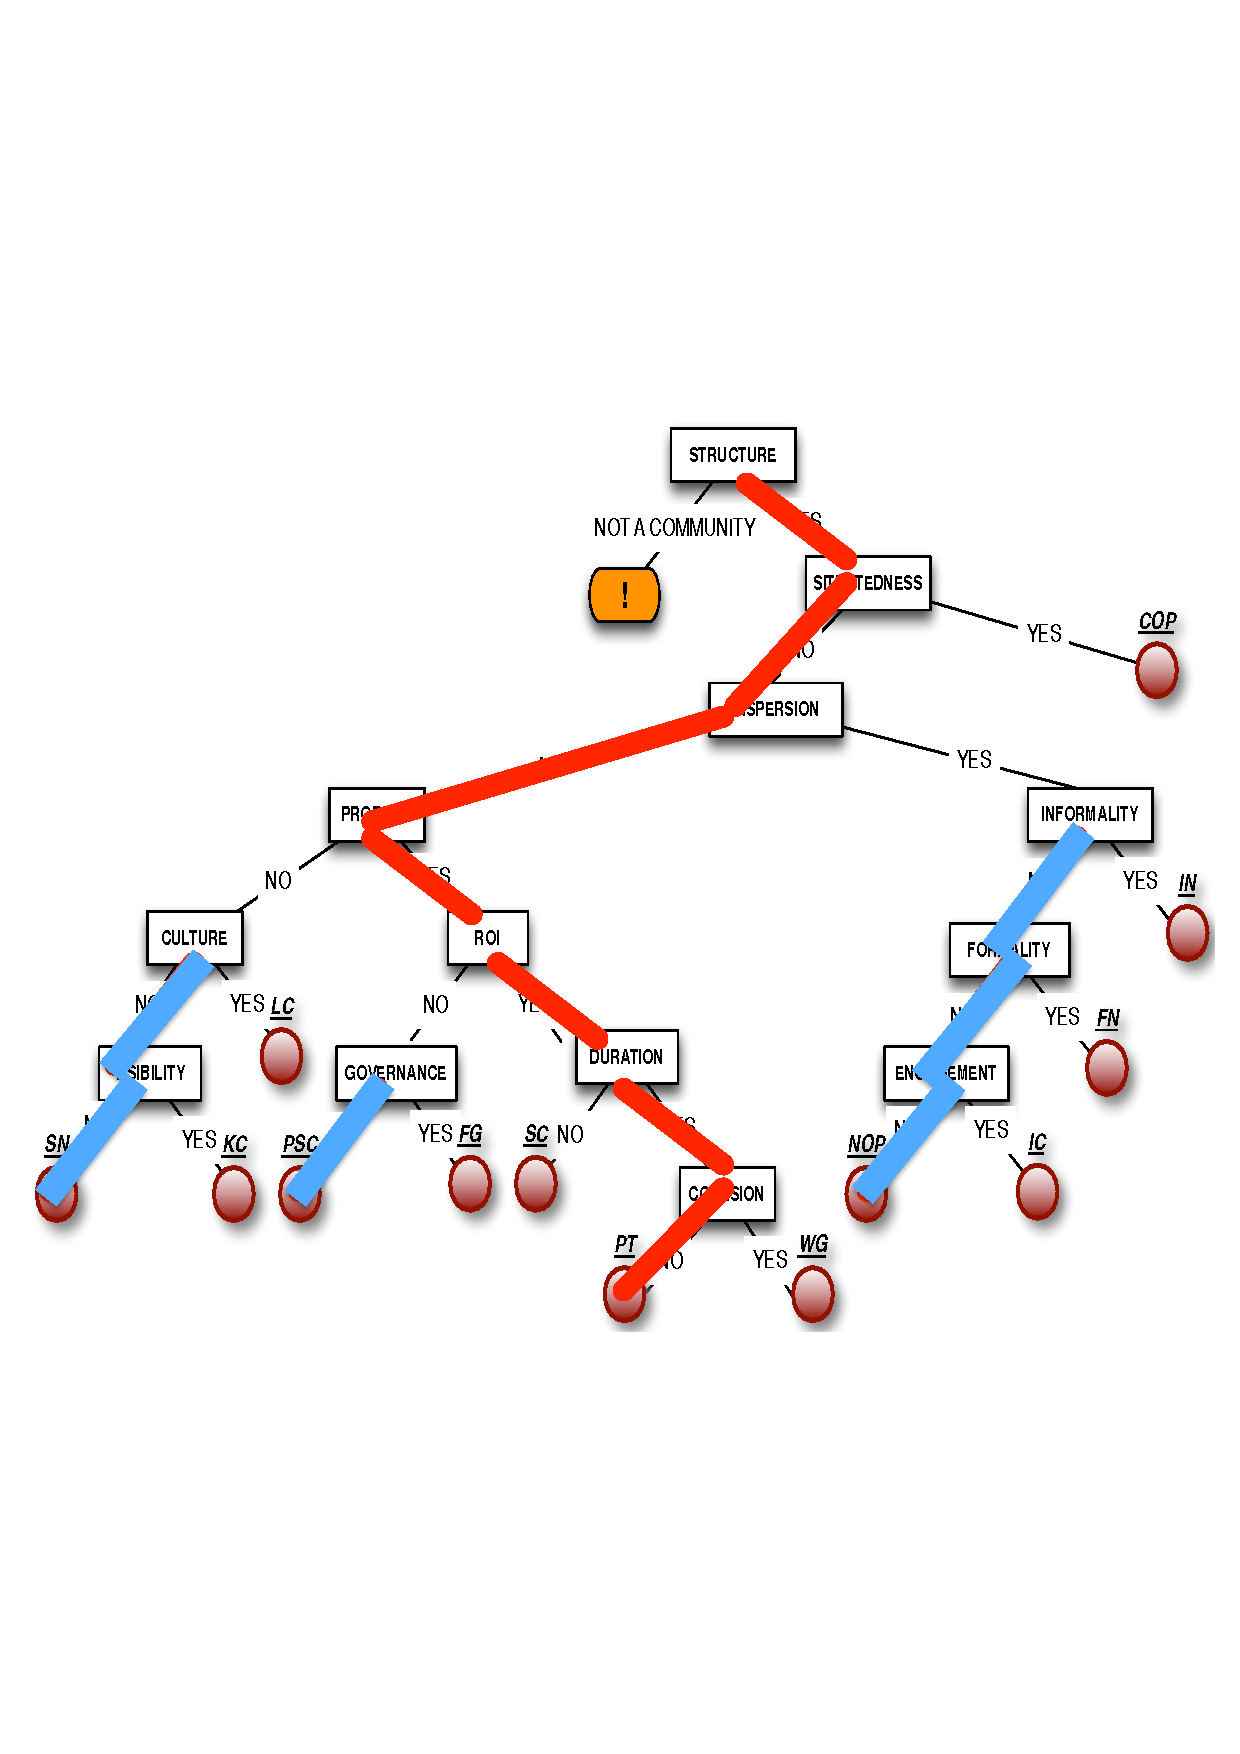
\includegraphics[width=5in]{coloring}%
%\end{sideways}
\caption{an example \emph{snapshot} for text-book project teams.}\label{snapshot}
\end{figure}
Applying SEEDS, we made three key observations: (a) the method allows uncovering inconsistencies on the observed \emph{snapshot}; (b) the community \emph{snapshot} can have a limited number of possible forms, each with its own particular characteristics; (c) the method allows uncovering undesirable properties that can hinder communication/collaboration across communities during software development. 

While based on previously published work, our paper offers the following novel contributions: (a) the SEEDS method, validated through a large industrial case-study; (b) a questionnaire and checklist that feature feedback from industrial practitioners; (c) analysis guidelines that allow to interpret the \emph{\emph{snapshots}} found - guidelines were obtained applying SEEDS in practice and feature feedback from industrial practitioners. 

The rest of the paper is structured as follows: Section \ref{devcomm} explains related work; Section \ref{mm} explains materials and methods; Section \ref{method} presents SEEDS; Section \ref{cs} validates SEEDS applying it no a large industrial case-study, while Section \ref{disc} discusses both contributions, namely SEEDS and its application. Finally, Section \ref{conc} concludes the paper with future work.

%these forms are worthy of further study since they could act as proxies for quality of the observed community.
%In addition we suggest ways to manipulate the community state, e.g.~to change community type or its focus. 
%In algorithms theory, a process state is given by the (current) values of all variables within the scope of the process \cite{algos}.
%Our method is based on empirical evidence. 

%%%%%%%%%% NOOOOOO!!!
%We found that a \emph{social community} is a specific type of social network for which certain attributes remain constantly true.

%We found that the status of a community is given by a set of paths on a community decision-tree.
%For example, imagine you are working within a UK open-source forge that collaborates with another open-source community from the US. This basic information conveys two critical informations: (a) the resulting community (US+UK) is \emph{dispersed}, i.e.~not collocated; (b) the resulting community is \emph{informal}. According to \cite{ossslr,specissue} the presence of these two attributes is necessary and sufficient to identify an \emph{Informal Network} social community type.
%

%Finally, we compare the identified social community attributes (i.e.~the community state) with empirical results from previous work \cite{ossslr}. This last step allows us to understand what can be done to improve the communities, e.g.~by encouraging changes in attributes.
%The benefits of using our method are threefold: first, practitioners can use the questionnaire as a checklist for missing management information; second, the questionnaire can be used as a guideline to engineer communities for a specific software development problem; third, the community state we obtain can be cross-referenced with development velocity to evaluate community effectiveness in the current state.
%\begin{figure*}
%\hspace{.5cm}
%%\begin{sideways}
%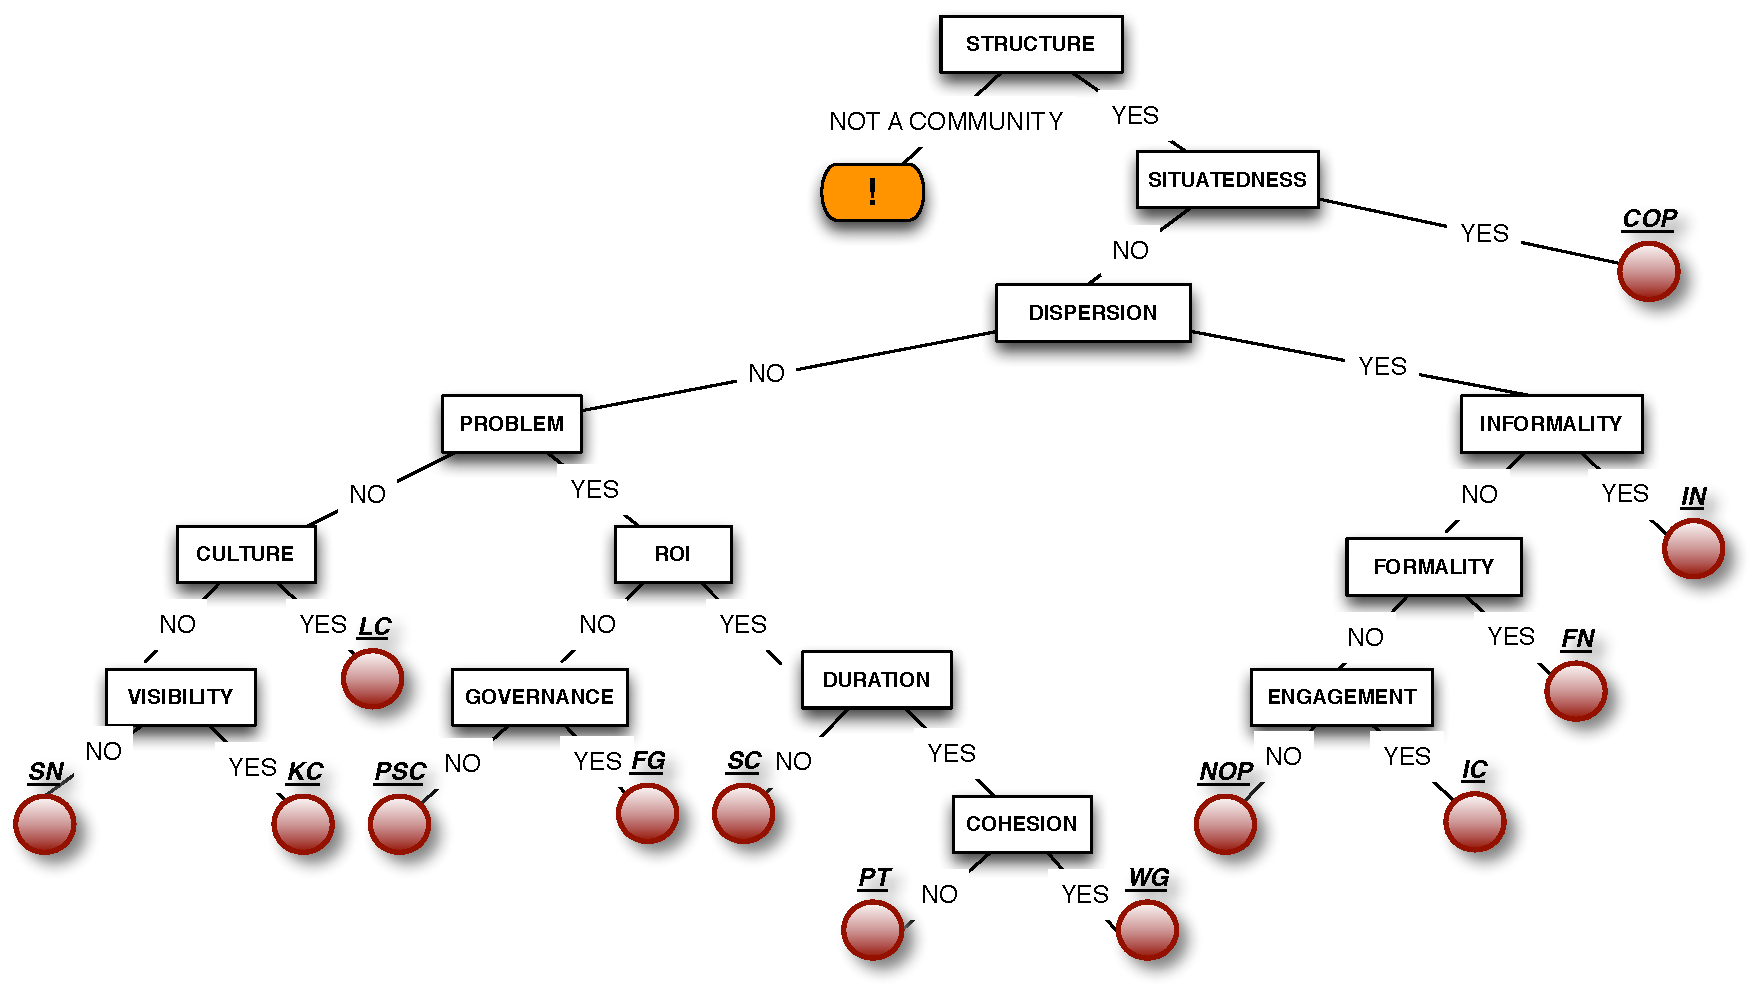
\includegraphics[width=6.3in]{tree}%
%%\end{sideways}
%\caption{a decision-tree to uncover social communities \cite{specissue}}\label{tree}
%\end{figure*}
%%

% no \IEEEPARstart
%This demo file is intended to serve as a ``starter file''
%for IEEE conference papers produced under \LaTeX\ using
%IEEEtran.cls version 1.7 and later.
%% You must have at least 2 lines in the paragraph with the drop letter
%% (should never be an issue)
%I wish you the best of success.
%\hfill mds

\section{Previous and Related work: Supporting Software Development Communities}\label{devcomm}

This section outlines work relevant to sustain the foundations of the material presented in this paper. In addition, we investigate on relevant research efforts related to our own.
%\begin{itemize}
%\item related work from socio-technical congruence
%\item related work dana damian
%%\item conway's law?
%\item other works in ged for social studies
%\item productivity and agile methods to be adopted in gsd
%%%%\end{itemize}
%%%TODO:\\
%%%RESTRUCTURE DIVIDING THE VARIOUS LITERATURE SECTIONS\\
\subsection{Previous Work}

In previous work we found that observable \emph{social communities}, e.g.~as captured in \cite{Davenport2001} are a composition of known social community archetypes \cite{ossslr}. Each community type can be given a distinct characterisation through key observable properties. The combination of these properties can be used to ``plot'' a community shape as well as study its performance. In \cite{ossslr} we presented an overview of the state of the art in social communities, offering a distinct characterisation for each type. The state of the art is summarized on table \ref{commtypes}.
The work presented in this paper goes one step further in this direction, by introducing a method to ``\emph{snapshot}'' software development communities. The method draws motivation and foundations from the works in \cite{icgseoss,ossslr} and uses results from \cite{specissue}. More in particular, data from \cite{ossslr} led us to work out a checklist of the key information that needs to be available to study a community. Data and reasoning in \cite{specissue} led us to work-out a questionnaire that can be used to both gather the data and analyse it, to obtain a community ``\emph{snapshot}''. Finally, the method inherits from \cite{specissue} the decision-tree which is essential to producing the community ``\emph{snapshot}''.

\begin{table}
\vspace{-2.5cm}
\hspace{-2cm}
\begin{tabular}{|>{\raggedright}p{2.4cm}|>{\raggedright}p{13.7cm}|}
\hline 
\textbf{Name} & \textbf{Description}\tabularnewline
\hline 
Communities of practice (COP) & {\footnotesize A CoP consists of groups of people who share a concern, a set of problems,
or a passion about a topic or practice. These people deepen their knowledge and expertise
in their topic or practice by interacting frequently, face-to-face, collaboratively (helping each other) and constructively (to increase their mutual knowledge). This set of social processes is called situatedness \cite{situated,Ruikar2009}.} \tabularnewline
\hline 
Informal Networks (IN) & {\footnotesize INs can be seen as loose networks of ties between individuals that
happen to come in contact in the same context. The driving force of
the informal network is the strength of these ties between members.
Finally, an IN differs from other types since it does not use governance
practices but its success is solely based on the cohesion of
its members \cite{Cross2005}.} \tabularnewline
\hline 
Formal Networks (FN) & {\footnotesize Within FNs, members are rigorously selected and prescribed. They are
forcibly generated and acknowledged by management of the network itself.
Direction is carried out according to corporate strategy and its mission
is to follow this strategy \cite{ossslr}.}\tabularnewline
\hline 
Informal Communities (IC) &{\footnotesize ICs are usually sets of people part of an organisation, with a common
interest, often closely dependent on their practice. They interact
informally, usually across unbound distances, frequently on a common
history or culture (e.g.~shared ideas, experience etc). The main differ-
ence they have with all communities (with the exception of NoPs) is
that their localization is necessarily dispersed so that the community
can reach a wider audience \cite{ossslr}.}\tabularnewline
\hline 
Networks of Practice (NOP) & {\footnotesize A NoP is a networked system of communication and collaboration that
connects CoPs (which are localized). In principle anyone can join
it without selection of candidates (e.g.~OpenSource forges are an
instance of NoP). NoPs have a high geodispersion, i.e.~they can
span geographical and time distances alike. The high geodispersion
increases their visibility and the reachability by members. An unspoken
requirement for entry is the expected IT literacy of members \cite{Ruikar2009}.} \tabularnewline
\hline 
Workgroups (WG) & {\footnotesize WG are groups of technical experts whose goals span an entire business area or array of
organisational factors. WGs are always accompanied by a number of organisational sponsors and are expected to generate benefits as wide as their goals. What\textquoteright{}s also fundamental, is that
a WG is always acknowledged and supported by organisational sponsor(s).}\tabularnewline
\hline 
Project-Teams (PT) & {\footnotesize PTs are made by people with complementary skills who work together
to achieve a common purpose for which they are accountable. They are
enforced by their organisation and follow specific strategies or organisational guidelines (e.g.~time-to-market, effectiveness, low-cost,
etc.). Their final goal is delivery of a product or service which
responds to the requirements provided \cite{ossslr}.} \tabularnewline
\hline 
Strategic Communities (SC) & {\footnotesize SCs consist of meticulously selected people, experts in certain sectors
of interest to a corporation or or a set of organisational partners
tied with formal non-disclosure agreements. These try to proactively
solve problems within strategic business areas of the organisational
sponsor.} \tabularnewline
\hline 
Formal Groups (FG) & {\footnotesize FGs are comprised of people which are explicitly grouped by corporations
to act on (or by means of) them (e.g.~governing employees or ease
their job or practice by grouping them in areas of interest). Each
group has a single organisational goal, called mission (governing
boards are groups of executives whose mission is to devise and apply
governance practices successfully). In comparison to Formal Networks,
they seldom rely on networking technologies, on the contrary, they
are local in nature.} \tabularnewline
\hline 
Problem-solving Communities (PSC) & {\footnotesize PSCs can be seen as a specific instance of a Strategic Community focused
on a particular problem. One would expect this community to be formal
in nature. Contrarily we found that they emerge as informal, since
informality aids brainstorming and problem-solving processes.} \tabularnewline
\hline 
Learning Communities (LC) & {\footnotesize LCs provide a space for pure learning and explicit sharing of actionable
knowledge (i.e.~skills). In a learning community, the leadership is
expected to steer the community\textquoteright{}s practices and membership
is subject to approval and tied to the learning objectives given to
the member. Each developed or exchanged practice must become part
of the organisational culture \cite{Ruuska2003}.} \tabularnewline
\hline 
Knowledge Communities (KC) & {\footnotesize KCs are groups of people with a shared passion to create,
use, and share knowledge for tangible business purposes (e.g.
increased sales, clients profiling, etc.).
The main difference with other types is that KCs are expected (by
the corporate sponsors) to produce actionable knowledge (knowledge
which can be put to immediate action e.g.~best-practices, standards,
methodologies, approaches, problem-solving-patterns, etc.) into a
specific business area \cite{ErikAndriessen2005}.} \tabularnewline
\hline 
Social Networks (SN) & {\footnotesize SNs represent the emergent network of social ties spontaneously arising
between individuals who share, either willingly or not, a practice
or common interest on a problem. SNs act as a gateway to communicating
communities \cite{Cross2005}.} \tabularnewline
\hline 
\end{tabular}
\caption{social community types, an overview.}\label{commtypes}
\end{table}

\subsection{Related work: Organizational Structures and Their Impact on Software Quality}
Literature in GSE already recognises the need to study global communities. More in particular, many works such as \cite{nachiappan} have studied empirically the effect of organisational structures on the quality of software. These works motivate further studies to understand, represent and support social structures and communities. In addition, similar works such as \cite{uls,rel9} study the effect of socio-technical congruence on designing global systems as well as the process of global engineering. Such works suggests that understanding how coordination requirements map to their people counterpart is critical to steer information across global communities successfully. Our work is limited to identifying community types, and finding ways to ``format'' and study their observable characteristics. 
Other works such as \cite{Davenport2001} study the impact of successful communities on socio-technical problems (e.g.~coordination, shared understanding, etc.). These works take a more social and organisational approach, pointing out the paramount importance of supporting explicitly the work of communities rather than allocating tasks to single individuals. 
%In addition, works such as \cite{scrum} study the impact of agile methods on a large scale distributed software engineering attempt. Understanding the impact and changes on global communities forced in by organisational changes such as agile adoption, is key to successful change, especially on a global scale.
%Our work in this paper does not go deep in investigating the impact of organisational decisions on the development community, but introduces a method to understand the community by \emph{snapshot}ting its current status. The method can be used to support related organisational decisions such as agile adoption. Moreover, the method enables understanding the negative consequences of change, such as emergent organisational barriers \cite{Correia2010}.
Finally, works such as \cite{rel,rel4} investigate the impact of organizational decision-making on software development. For example, understanding if the current community \emph{snapshot} is performant (or even compatible) with offshoring is essential for the community to ``go global'' \cite{icsesympo}. The method presented in this paper can be used to support organisational decisions, investigating the current and to-be community \emph{\emph{snapshots}}. Finally, the method enables understanding the negative consequences of change, such as emergent organisational barriers \cite{Correia2010}.

\subsection{Related work: Organizational Governance for Global Software Development Communities}

%%%INCLUDE MORE LITERATURE ON GOVERNANCE AND RELATED WORK\\
%%%INCLUDE MORE LITERATURE ON HUMAN ASPECTS IN SE\\

\subsection{Related work: Networked and Agile Organizations}

%INCLUDE EVIDENCE OF ORGANISATIONAL CHANGE AND GOVERNANCE AS A CONSEQUENCE OF AGILE METHODS\\

%
%
%TODO: elaborate with the rest of related work, e.g.~references on organisational change, other empirical studies in global communities or global communication \\
%
%\subsection{Research Questions}\label{rq}
%
%This paper reports an empirical study of software development organisations. We pay particular attention on the layout of the organisation. Our work was driven by the following research questions:
%
%\begin{center}
%{\bf What elements of a development community should be made explicit to study its instantaneous state?}
%\end{center}
%Previous research in organisational studies, social-networks analysis (SNA) and software engineering, suggest there are many variables at play within a software development community. In previous research \cite{ossslr,specissue}, we provided an extensive specification of attributes that define community types. Table \ref{commtypes} provides an overview of community types. These types were obtained through a Systematic Literature Review on organisations and social-networks research \cite{ossslr}. In this work we present information essential to define a \emph{snapshot} for an observed organisation. By examining interviews and other sources of organisational evidence, we found a way to represent a \emph{snapshot} of an observed community, such that the \emph{snapshot} can be further analysed.
%
%\begin{center}
%{\bf What are the possible forms of the development community \emph{snapshot}?}
%\end{center}
%In previous work \cite{icgseoss,specissue} we found many combinations of communities that can represent software development.
%%Studying interviews and analysing grounded-theory results from available organisational data, we found the possible forms that a community status can assume. Each of these forms manifests with own characteristics and should be acted upon accordingly.
%In this work we analysed the possible ``colourings'' of the decision-tree in \cite{specissue} using data from a big industrial case-study as a reference. We found there are four possible ``colourings'' that the data can reflect.

%
%\begin{center}
%{\bf How does organisational change influence the form of a development community \emph{snapshot}?}
%\end{center}
%Much research is aimed at establishing the influence of organisational change on the people and process of software engineering. For example, In previous work \cite{specissue}, we found that the ``shift'' to agile methods could be an organisational change with both positive and negative impact. The organisation we studied was undergoing an organisational ``shift''. Studying the opinions of developers and technicians, and the characteristics of the community \emph{snapshot}, we found barriers that clashed with the success of organisational change.

%\begin{itemize}
%\item explain impact of the question and importance of answering
%\end{itemize}
%%%%%%%%%%Providing an intelligible shape for an observable software development community is the first step towards efficient steering of community operations. 
%%%%%%%%%%
%%%%%%%%%%For example, studying \emph{snapshots} of global communities enables the development of ad-hoc adaptations based on current (or desired) community \emph{snapshots}. Global software development literature acknowledged that global communication is compromised by the presence of organisational barriers within and between communities \cite{gse,gsdbook}. Given the presence of barriers in certain \emph{snapshots}, organisations could plan organisational adaptations to those barriers.
%%%%%%%%%%
%%%%%%%%%%Moreover, studying \emph{snapshots} of communities, managers can plot cross-community communication patterns that match exactly the current situation. For example, during a Scrum sprint, Scrum coaches can evaluate \emph{snapshots} of the development community to understand its productivity and adapt it as needed (e.g.~to avoid ``Crunch-times'' in Scrum).

%
%previous research in software engineering, organisational sciences and systems theory has observed many social community types. Over time, many attributes were observed and used to characterise these community. We analyse empirical evidence with the aim of pinpointing the attributes that are necessary and sufficient to capture the state of a certain community
%
%Second, {\bf how can we act on the status of a software development community?}  .\\
%
%Finally, {\bf how can practitioners use the state-of-the-art in social communities to improve development collaboration?}  .\\

% 
%\hfill January 11, 2007
%
%\subsection{Subsection Heading Here}
%Subsection text here.
%
%
%\subsubsection{Subsubsection Heading Here}
%Subsubsection text here.
%

\section{Materials and Methods}\label{mm}
%This paper introduces a method to study a development community using a case-study. 
The conclusions in this paper are drawn from a real-life industrial case-study. This section explains what materials we used to carry out the case study and how we examined such materials.

\subsection{Materials}
%TODO: explain that two people conducted the case-study with the same material in parallel with minimal interaction on the case study, as overseen by two senior researchers. when it was finished the results were compared for evaluation. the method can be generalised since both researchers followed the same emergent path and encountered the same probs, that were solved in pretty much the same way.\\
%The following sections describe materials and methods in more detail.

%\begin{itemize}
%\item describe work in the SLR
%\item describe work in ICGSE paper
%\item describe work in IEEE Sw paper
%\item related work
%\end{itemize}
%
%\subsection{Materials Used}
The empirical evidence used in our work, stems from empirical research conducted in a big organisation, active in the mobile technologies market. The organisation (called Company X from now on) is multinational that develops both hardware and software components for end-users' mobile-phones and apps to enrich user experience. Company X employs over 130K people in 16 worldwide sites, with sales in over 160 countries. At the time the empirical research was conducted (early 2012), the organisation had a net market sale of 42.4 billion euros. 

The focus of our data lies in the organisational structure of a product-chain within Company X's corporate portfolio. Our empirical data describes the overall organisation and some of its software development sites. The data also reports on the collaboration between Company X's Scrum development community and a constellation of open-source communities. 

Three key sources of evidence were used:
\begin{enumerate}
\item The first key resource (called \emph{\bf Reference 1} from now on) is a research report studying agile and open-source adoption in Company X. The study was conducted using grounded-theory \cite{gt}. The study features six interviews with focus groups from Company X. Focus groups had varied expertise, from areas such as project management to agile coaches to code developers. The focus sessions are analysed through grounded theory. The study offers an overview of the organisational structure of Company X as a whole (i.e.~as a global community) as well as explaining its local sites. The research focuses on a division of Company X, working on a specific project release, at the time of investigation. The report is 112 pages long, we use page numbers for the purpose of traceability. 

\item The second key resource (called \emph{\bf Reference 2} from now on) is a research report studying three software engineering teams within Company X. The study features 16 interviews harvested through accidental and snowball sampling \cite{Goodman}. Interviewees had varied backgrounds but an average work experience in Company X of about 10 years. The sample consisted of both sexes, however, with a minority of females. As a result, the organisational details of this report focus around software process, software coding methods, development best-practices adopted, problems found, and ultimately, the people's perspective on all the above. The report is 97 pages long, we use page numbers for the purpose of traceability.

\item The third key resource (called \emph{\bf Agile Slides} from now on) is a set of tutorial slides that agile coaches within Company X used to introduce X's organisational structure/process to newly appointed staff members. The slides provide an overview of the agile process and open-source integration protocols in place within Company X at the time of investigation. The report is 4 pages long, we use page numbers for the purpose of traceability.

\end{enumerate}

One of the agile coaches in the case organization was able to give continuous feedback throughout the research and the writing of this report. This person clarified the structures and working modes inside Company X and provided deeper insight into one of the departments (the same covered by Ref.~2). We are therefore confident that our interpretations of the key sources of evidence are essentially correct.

All of the above sources are dated around 2012 and describe the company as it was in 2010 or 2011. The sources are protected by non-disclosure agreements\footnote{Available upon signed request.}. At the time of investigation, Company X was going through many organisational changes and both studies aimed at understanding the impact of organisational change on teams, their production velocity, community productivity and end-product quality. 

\subsection{Research Methods}
%TODO:\\
%ALSO SPECIFY HOW WE ARRIVED TO THE SEEDS METHOD\\
%BTW HOW DID WE ARRIVE TO THE ODESS METHOD?\\
%CYNEFIN TO CROSSREFERENCE RESULTS AND FINDINGS\\

We elaborated SEEDS starting with a gap analysis of previous results. Through brainstorming and evaluation by an industrial partner we were able to obtain a revised version of the method. Finally, to validate SEEDS we conducted a case-study following guidelines in \cite{runeson}. \\
%ELABORATE\\
%Given the same input materials, two parallel case-studies were started, with 
The case-study objective was to evaluate real-life development communities from a big industrial case using results from previous work \cite{specissue}. The work in \cite{specissue} presents a decision-tree that allows to identify community types (summarised on Table \ref{commtypes}) by means of key defining attributes. 
%
%The study was intended to validate and enrich the method from our previous work, to make it usable in real-life practice. 
Besides providing validation to the decision-tree in \cite{specissue}, the connotation of our case-study was exploratory and descriptive. We set out to define an intelligible form for the observed development community, such that the outlined form could be further studied, e.g.~compared to organisational metrics for Company X. These followup quantitative studies are out of the scope of this work.

%
%After our analysis was done, we explored the generality of our approach and findings, by comparing results from both parallel studies. We found that both efforts were carried out with the same underlying approach. We concluded that the approach can be generalised into SEEDS, a method to outline development social structures to analyse them by capturing \emph{\emph{snapshots}}. 

We used a parallel study (referred to as \emph{Sub-study 2}, from now on) and data sources triangulation \cite{stake} to tackle threats to validity, as discussed in Section \ref{disc}. The use of the \emph{Sub-study 2} parallel study was meant to minimise bias and unreliability of results through observer triangulation, according to \cite{stake}. The parallel case-study was conducted by an insider of Company X, using data available as well as his own expertise and experience/knowledge about Company X. While the two studies were started at the same time, the researcher conducting the first study (called \emph{Sub-study 1}) was prohibited to share increments of partial results. Weekly meetings were planned to assess progress status only. The supervision of two senior researchers was used throughout the duration of the study to assess the quality of progress.

%
%Moreover,  was used to aid the generalizability of our results. To this purpose, three different sets of data were used. Two of these were obtained through surveys and other empirical enquiry methods.
%
%using questionnaire to gather and organise organisational information needed plus the decision-tree to match with visits and comm. types use the piece below as a start\\
%
%
\section{The SEEDS Method}\label{method}

SEEDS entails using four practical tools: (a) a questionnaire; (b) a checklist; (c) a decision-tree; (d) an analysis framework. The remainder of this section introduces the SEEDS method in phases. Sections \ref{quest} to \ref{fw} provide additional details on the questionnaire, checklist, decision-tree and evaluation framework.
%

 \begin{figure}[h!]
%\hspace{-.6cm}
%\begin{sideways}
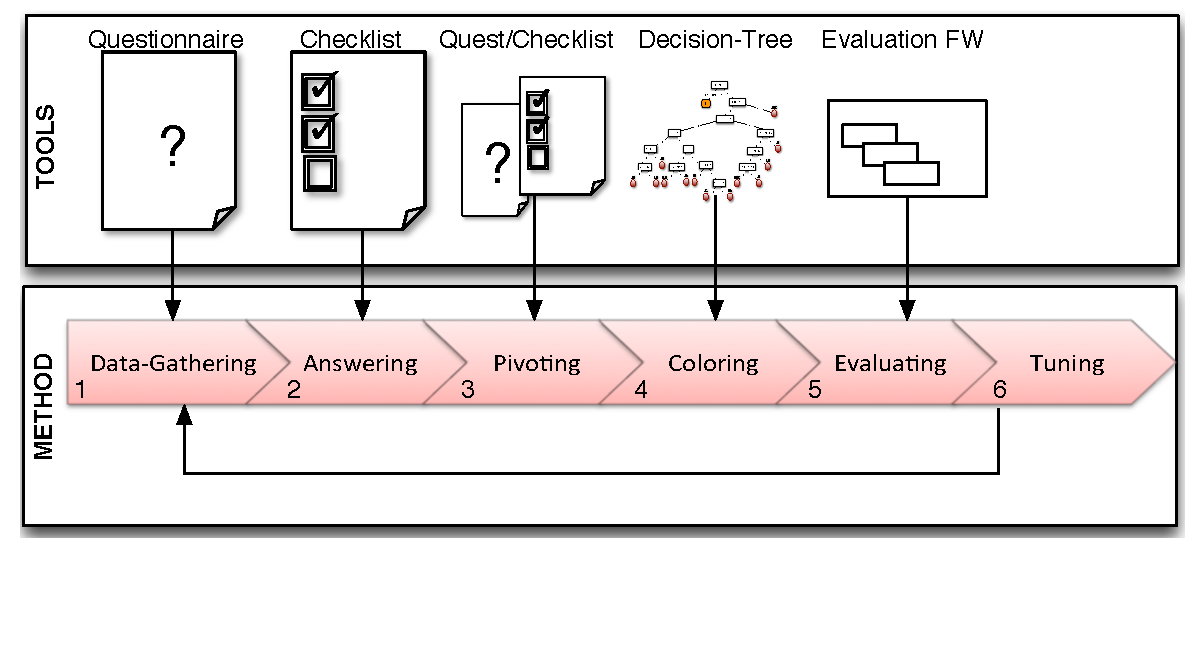
\includegraphics[width=5.3in]{odessamethod}%
%\end{sideways}
\caption{The SEEDS Method: Tools and Phases.}\label{SEEDS}
\end{figure}
%First, a checklist is used to gather the essential organisational data to characterise an observable community.  The questionnaire can also be fed to members of the observed community to gather the needed data.
%\subsection{Method Phases}
%ELABORATE\\
SEEDS unfolds in the following phases:

\begin{enumerate}

\item \emph{\bf Data-Gathering:} \emph{Use questionnaire to gather needed community data.}
Missing data can be gathered by directly surveying (e.g.~with online forms) members of the community under observation. Alternatively, quantitative mechanisms can be used, such as Social-Network Analysis (SNA) \cite{Rosso2009}. Table \ref{quest} presents the SEEDS questionnaire. Each question is the result of analysis and brainstorming sessions with industrial partners and other cooperators. The questionnaire refinement exercise was aimed at pinpointing the right questions for SEEDS.

\item \emph{\bf Answering:} \emph{Use checklist to get attributes value.}
The checklist must then be filled out using the data gathered through our questionnaire. The checklist is a lightweight mechanism to analysing observable development communities, rather than using complex coding schemes on available evidence, as seen previously in literature \cite{Hustad2010,Rosso2009}. Fig.~\ref{checklist} shows the list. Each item within the checklist is a key defining attribute for a community type (see Table \ref{commtypes}), according to data in \cite{ossslr}. Available data must enable answering all the questions in the questionnaire.

\item \emph{\bf Pivoting:} \emph{Double-check questionnaire and checklist to identify multiple answers.}
Pivot-points are points in the checklist that can have multiple answers. A community is a fluid, dynamically evolving emergent property of cooperating organisations. We found in practice multiple community archetypes emerging at the same time where managers assumed there were none. Pivot-points indicate either: (a) there is a conflict or inconsistency in the analysed community \emph{snapshot}; or (b) another community (or sub-community) exists within the observed community, strong enough to cause conflicts and inconsistencies. For example an observed community might show both ``dispersed'' sites and ``non-dispersed'' sites. This means that the community is the sum of multiple communities, based on the remaining attributes.

\item \emph{\bf Coloring:} \emph{Use checklist to ``color'' the SEEDS decision-tree.}
Answers from the checklist allow immediate mapping to the decision-tree to uncover community types and additional attributes present in the observed community. A community \emph{snapshot} has been obtained.

\item \emph{\bf Evaluating:} \emph{Use evaluation framework to analyse the \emph{snapshot} found.}
The framework shown in Fig.~\ref{fwpic} provides a lens to interpret the \emph{\emph{snapshots}} from multiple angles. More in particular, the framework allows to pinpoint hazardous organisational barriers and assist in organisational decision-making by means of the \emph{snapshot}. For example, the evaluation framework allowed us to discover a hazardous communication barrier and the means to mitigate it.

\item \emph{\bf Tuning:} \emph{Use evaluation and literature \cite{ossslr} to act on the community.}
\emph{\emph{Snapshots}} can be evaluated to steer community operations. SEEDS allows to pinpoint critical information with which to act on the community, by ``tuning'' desired properties. For example, in practice we found an organisational barrier that can be mitigated by adding a knowledge community within the analysed \emph{snapshot}.

\end{enumerate}
\begin{table}
\hspace{1cm}
%\begin{sideways}
%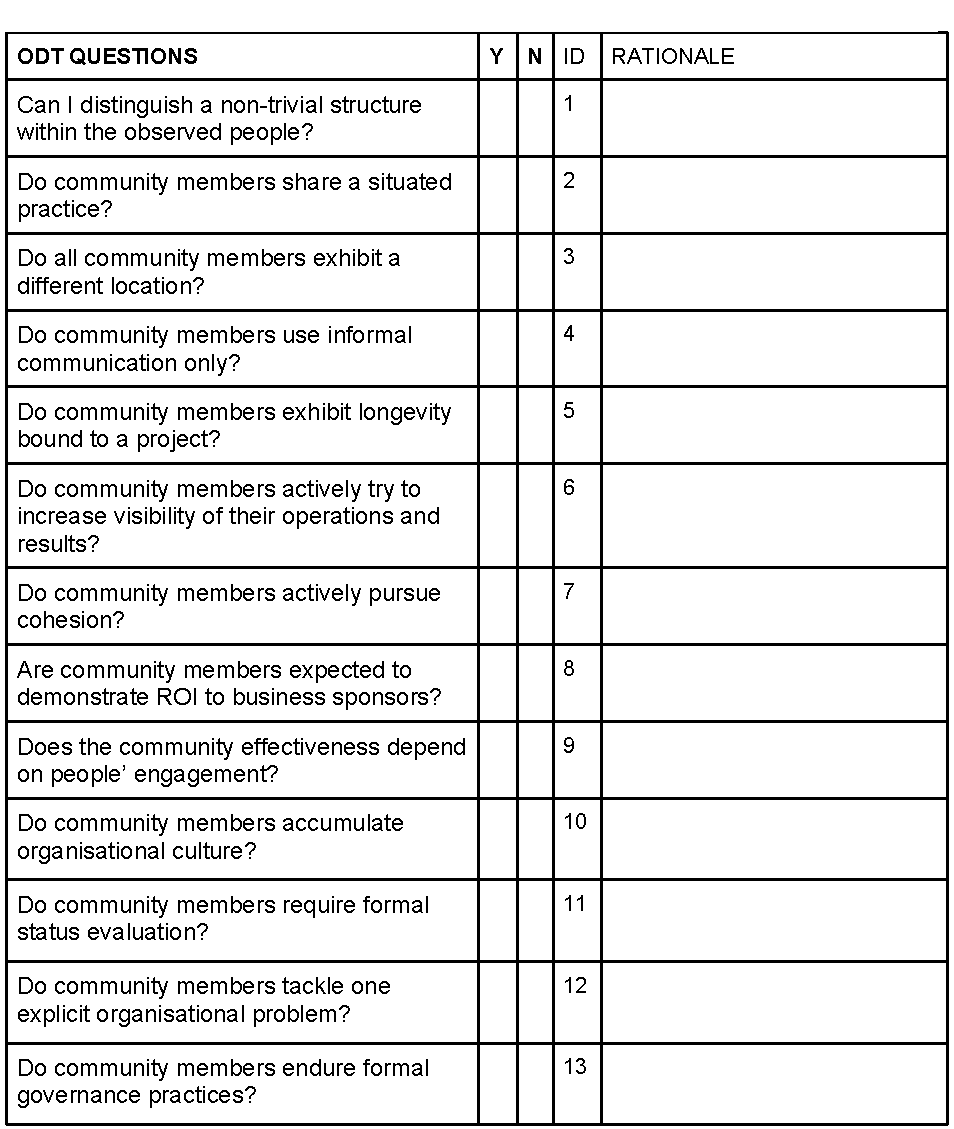
\includegraphics[width=5.44in]{quest}%
%\end{sideways}

\begin{tabular}{|>{\raggedright}p{11cm}|>{\raggedright}p{1.5cm}|}
\hline 
\textbf{Question} & \textbf{Answer}\tabularnewline
\hline 
\emph{Can you distinguish an organised structure across yourself and
your colleagues?} & \tabularnewline
\hline 
\emph{Do you and the colleagues you work with work in the same single
site?} & \tabularnewline
\hline 
\emph{Do you work in a highly-distributed setting with few teams or
colleagues per location?} & \tabularnewline
\hline 
\emph{Do you and your fellow colleagues interact informally only?} & \tabularnewline
\hline 
\emph{Do you work on time-bound projects?} & \tabularnewline
\hline 
\emph{Do you and your colleagues disseminate or increase the visibility
of your work? } & \tabularnewline
\hline 
\emph{Do you and your colleagues actively try to team-build? } & \tabularnewline
\hline 
\emph{Do you need to explicitly demonstrate ROI to your organization? } & \tabularnewline
\hline 
\emph{Does the success of your community depend on your engagement? } & \tabularnewline
\hline 
\emph{Do you and your colleagues actively gather and share organisational
culture (e.g.~best-practices, common problems)?} & \tabularnewline
\hline 
\emph{Were you and your colleagues formally evaluated and qualified
when enrolled in the organisation? } & \tabularnewline
\hline 
\emph{Do you and your colleagues work against the same specific organisational
problem? } & \tabularnewline
\hline 
\emph{Do you and your colleagues undergo rigid governance models imposed
by your organisation? } & \tabularnewline
\hline 
\end{tabular}
\caption{The SEEDS Questionnaire.}\label{question}
\end{table}

Figure \ref{SEEDS} provides an overview of SEEDS. The method starts by using the questionnaire, proceeds by applying a checklist and map results to a decision-tree. Finally, the method assumes analysis and action are performed through the obtained \emph{snapshot}.
%%TODO:\\
%%FIGURE IS IN PROGRESS\\
%%%%% SONO ARRIVATO QUI

\subsection{The SEEDS Questionnaire}\label{quest}

We produced and refined a questionnaire that can be used to gather necessary details directly from the members of the observed community. Questions were elaborated stemming from lessons learned in \cite{specissue} and refined through feedback by industrial and academic partners. Each question in the list produces data to pinpoint the existence of key community attributes.


\subsection{The SEEDS Checklist}\label{cl}

As part of the work in \cite{ossslr} we analysed 143 articles discussing social communities in the areas of software engineering, organisational studies and social networks. We found many different definitions for social community types. Some articles discussed a type X as defined in previous literature, but added new attributes for that type. Other articles introduced new values for an attribute of X. 

To characterise different social community types using this empirical evidence, we studied and compared all definitions available for each type. 
We began this process by isolating attributes common to all articles discussing a certain type. 
Then we divided common attributes of each type into two groups: (a) attributes with more than one possible value; (b) attributes whose value was fixed. 
We found that, for most types, group (a) counted many elements and many values. Conversely, group (b) were populated by a single element for each type. 
From this, we made two key observations. 
First, the singletons in groups (b) uniquely identify a type.
Second, combining groups (a) and (b) together characterises the community type. We named the singletons in groups (b) as \emph{key-defining} attributes.

The checklist in \ref{checklist} contains \emph{key-defining} attributes for community types. Filling the checklist (using data in the questionnaire) allows using it to ``colour'' the decision-tree.

The checklist begins with the STRUCTURE attribute. This attribute is the \emph{key-defining} of social-networks \cite{ossslr}. We found that a community can be seen as a specialised version of a social-network for which certain conditions and social arrangements are constantly true. This is why the first decision node ascertains the presence of a (organisational) structure among the observed set of people. This first property is keyed in a very simple, yet fundamental, axiom: ``a \emph{social community} is an emergent property, i.e.~a characteristic by virtue of which, the \emph{whole} might be different than the sum of its \emph{parts}''. To decide this property you need to be able to distinctly observe a ``whole'' (called macrostructure) and its ``parts'' (called microstructures). However trivial it might seem, without this essential precondition, the observer would be faced with an unorganised crowd of people, without a structure, goal or observable characteristics. This notion could be assimilated with a demi-social-network made of nodes without links.

\begin{figure}[h!]
%\begin{wrapfigure}{r}{0.30\textwidth}
%  \begin{center}
    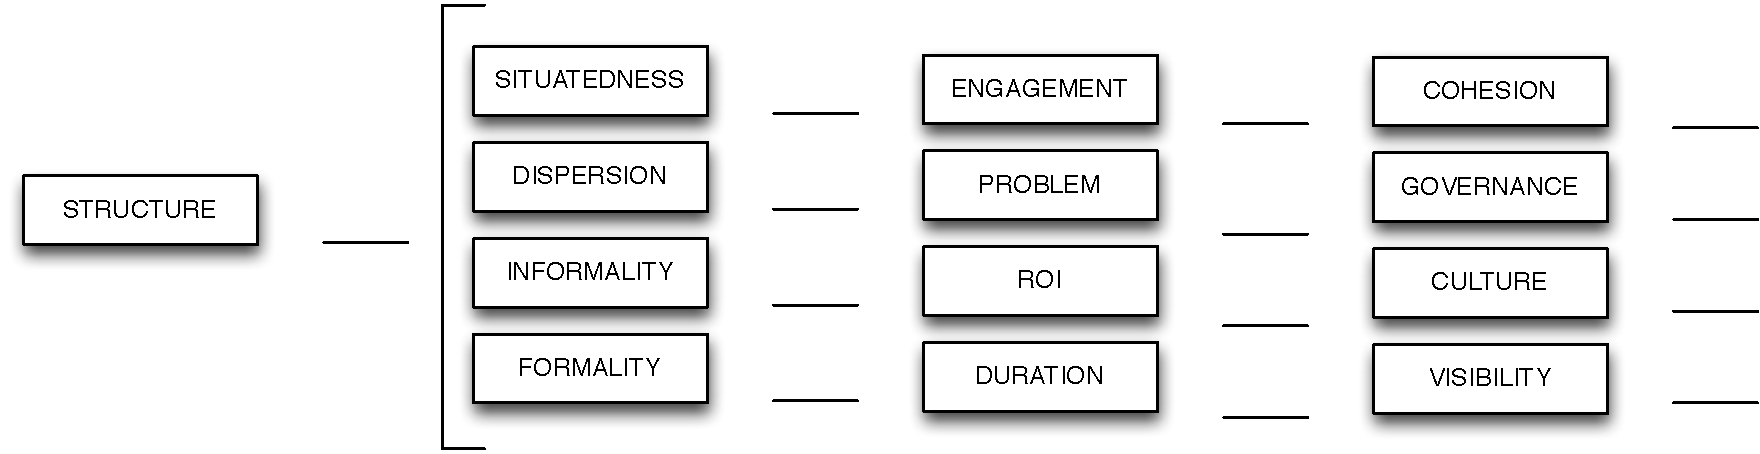
\includegraphics[width=5.3in]{checklist.pdf}    %
%  \end{center}
%\vspace{-.3cm}
\caption{\footnotesize SEEDS: a checklist for essential community information.}\label{checklist}
%\end{wrapfigure}
\end{figure}
\subsection{The SEEDS Decision-Tree}\label{dectree}

The notion of \emph{key-defining} attribute is not applicable to all cases. What happens if we observe multiple \emph{key-defining} attributes together in a real-life situation? We must then be able to relate this observation to the corresponding social community types. For this reason, SEEDS blends the checklist in Fig.~\ref{checklist} with the decision-tree in Fig.~\ref{tree}, from previous work \cite{specissue}.

Analysing the \emph{key-defining} attributes we found many relations between them: for example, some implied or mutually-excluded others. The relations formed a partial-order function for \emph{key-defining} attributes. A partial-order function associates an ordering or sequencing to the elements of a set. A real-life example of a partially-ordered set is a family genealogical tree, where some pairs of people bear the descendant-ancestor relationship, but not all pairs.

The decision-tree (see Fig.~\ref{tree}) is a representation of the partial-order relationship between \emph{key-defining} attributes. All the relations can be found online\footnote{\url{http://www.fileden.com/files/2012/3/7/3275239/OSSdecision.pdf}}.

The nodes on the tree are labelled with \emph{key-defining} attributes (e.g.~if a ``STRUCTURE'' and ``DISPERSION'' are observable then type NoP is identified). When visiting the tree, the observer needs to decide wether the key defining attributes are present or not. Each decision can be formulated in terms of a question (e.g.~``Do community members use informal communication only?''). These questions can be easily answered by observing any organisation, be it a single development effort, or an entire enterprise. 

The edges of the tree are Yes/No decisions made for each node, from the checklist (see Fig.~\ref{checklist}). 
The leaves of the tree are social community types (see Table \ref{commtypes}).

\begin{figure}[h!]
%\begin{wrapfigure}{r}{0.30\textwidth}
%  \begin{center}
    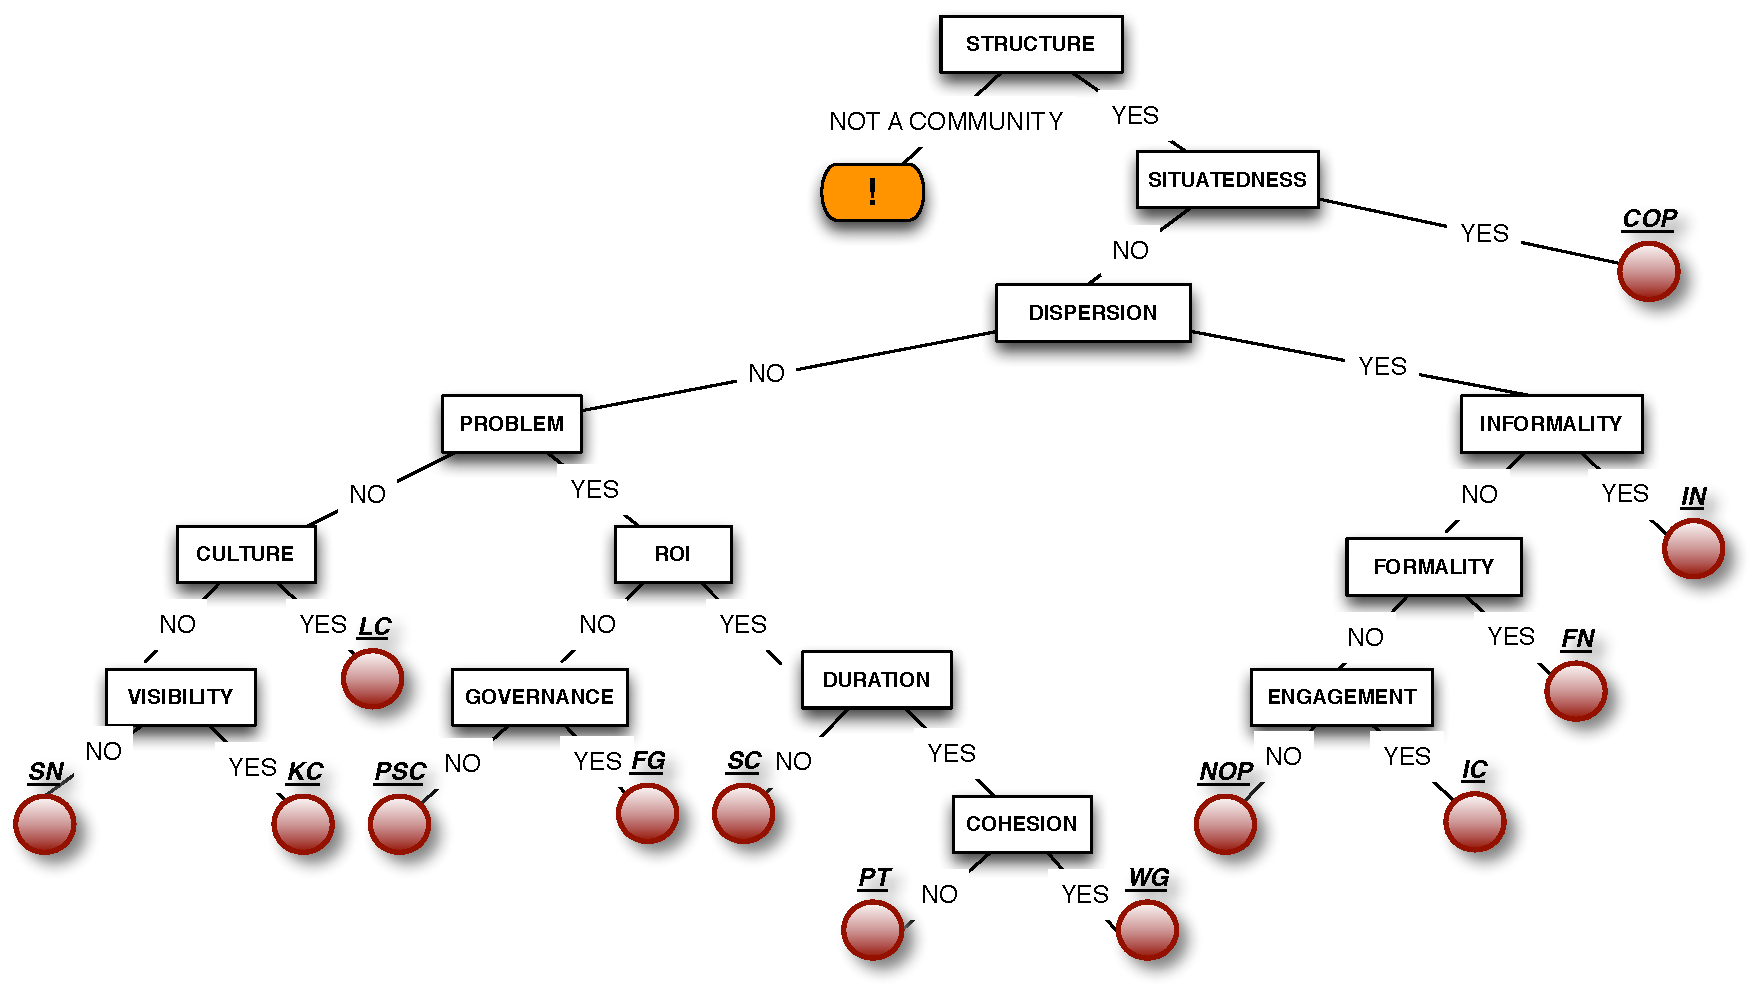
\includegraphics[width=5.3in]{tree.pdf}    %
%  \end{center}
%\vspace{-.3cm}
\caption{\footnotesize SEEDS: a checklist for essential community information.}\label{tree}
%\end{wrapfigure}
\end{figure}

\subsection{The SEEDS Analysis Framework}\label{fw}

Inheriting from strategic evaluation approaches such as \cite{swot}, we elaborated an initial analysis framework for SEEDS \emph{snapshots}. To understand strengths, weaknesses, opportunities and threats analysing community properties using SEEDS \emph{snapshots}, there are three key dimensions that must be evaluated.

First, observers must evaluate the \emph{snapshot} form; second, observers must find \emph{desirable properties}; third, finally, observers must verify if the observed community has \emph{higher-order needs}. Figure \ref{fwpic} shows the resulting evaluations that can be performed (on the left-hand side) using either decision-tree forms, desirable properties or higher-order needs (right-hand side).

SEEDS \emph{snapshots} can assume three possible forms:

\begin{enumerate}
\item \emph{Simple}: the answers in the questionnaire reflect a single, clear-cut path on the decision-tree. The community is well delineated and reflected by a type from literature. Additional attributes in the checklist are not present. The scenario exemplified earlier in Section \ref{intro} represents an instance of a simple community \emph{snapshot}. This form evidences a \textbf{strength} and \textbf{opportunity} of the community. The community is well defined and can be ``enriched'' with additional communities (or attributes) in a controlled fashion, e.g.~using additional SEEDS \emph{\emph{snapshots}}. This level of control delivers an advantage compared to other forms. Also, the company can expand the community as needed, using extensions to its advantage.

\item \emph{Enriched-Community}: the answers in the questionnaire reflect one path blended with additional attributes (including pivots) but no additional paths. This form evidences attributes that ``enrich'' the community, and can represent a \textbf{threat} for the community. The additional attributes can be caused by positive emergent circumstances but also harmful ``deviations''. This form can require additional study.
For example, suppose the ``visibility'' attribute is discovered in mix with the Formal Networks community type. Formality within formal networks might have forced the organisation to adopt mechanisms to increase the visibility of projects, people or artefacts, perhaps it is wise to foster the generation of a Knowledge Community jointly with the Formal Network. The enrichments indicate reasons for insufficient communities support. Practitioners can use the evidence to fill-in with missing support. Refinement and explicit support to such technologies includes the adoption of Information Management or Social Networking technologies \cite{eis,eim} to support development community.

\item \emph{Complex}: The answers in the questionnaire reflect more than one path through one (or more) pivot points. The \emph{snapshot} can be used to identify and support explicitly sub-communities. This form evidences possible \textbf{opportunities} for the community. Sub-communities can be identified by analysing deeper available pivots. Information leading to the ``multiple'' answer could be referred only to a specific division or location within the community. For example, suppose you analyse a Global Software Development organisation. Suppose you find a WG and DISPERSION is a pivot-point, that leads to the identification of a NoP. Details leading to a NoP however, when analysed further, are only referred to a single site in the GSD organisation. In case sub-communities are identified, managers can use the \emph{snapshot} to plan explicit support to their attributes.

%
%Pivot-points can also indicate reasons for an inefficient community. Community members show attributes of other communities that were not explicitly planned nor supported.
%\item \emph{complex}: The answers in the questionnaire reflect more than one path and additional attributes.
%\item \emph{chaotic}: The answers in the questionnaire reflect sparse attributes that don't represent any path but only broken segments. This indicates that the community is in some disarray, since it doesn't show any clear organisational form. The community is not representable with known organisational types. The \emph{snapshot} form can be used to identify the attributes that remain unsupported (i.e.~the broken links). For example, suppose you are observing a set of people working almost as a Workgroup but are not required to show any benefit on investments. This shortcoming can be made explicit and further investigated.
\end{enumerate}

% Ref to Ralph Stacey's certainty/agreement matrix. See the summary at http://www.gp-training.net/training/communication_skills/consultation/equipoise/complexity/stacey.htm
This division has many similarities to the Stacey matrix \cite{sta02aa}. We will explore this connection in Section~\ref{sec:complexity}.

Second, \emph{\mbox{(un-)desirable} properties} are items in the checklist that were (a) desired but not discovered, or (b) discovered but not desired. For example imagine you expected your community to exhibit increased visibility of its members and resources, but found the VISIBILITY attribute to be NO. This analysis reveals possible \textbf{weaknesses} of the community. Additional properties can be fostered with explicit supportive services (e.g.~using knowledge-bases or enterprise social networks to foster VISIBILITY). Conversely, imagine you found the attribute FORMALITY set to YES but expected there to be more informality in the way of working within your company, e.g.~to foster collaborativeness. Again, this analysis reveals \textbf{weaknesses} of your community. Left uncontrolled, some aspects of the community emerged an undesirable feature. This analysis dimension can be used to fine-tune community governance based on the properties found \emph{\mbox{(un-)desirable} properties}.

Third, finally, the decision-tree can be divided in three areas. 
\begin{enumerate} 
\item \emph{structure:} the first three nodes of the tree, namely STRUCTURE, SITUATEDNESS and DISPERSION, focus on the structure of your community, e.g.~whether it has a situated or dispersed practice.
\item \emph{networking:} the YES-branch out of the DISPERSION node, identifies community archetypes whose purpose is increasing the networking within your organisation or across partner organisations. The community's focus is networking, either autonomously or on-purpose.
\item \emph{goals:} the NO-branch out of the DISPERSION node, identifies community archetypes whose purpose is pursue a particular goal, under certain conditions. The community's focus is its goal (e.g.~an organisational problem or Return-on-Investments).
\end{enumerate}

The three areas or ``foci'' above, are higher-order properties of your community. SEEDS \emph{\emph{snapshots}} can be analysed to identify the missing focus, i.e.~a \emph{Higher-order need}. For example, imagine you take a \emph{snapshot} of your community and find out that the networking ``focus'' is missing but desired. You can use the \emph{snapshot} to identify the missing properties to pursue networking as desired.

\begin{figure}[h!]
%\begin{wrapfigure}{r}{0.30\textwidth}
%  \begin{center}
    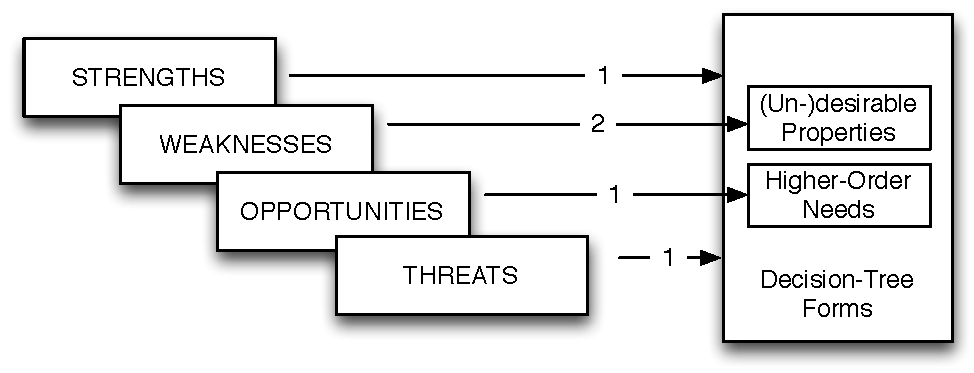
\includegraphics[width=5.4in]{fw.pdf}    %
%  \end{center}
%\vspace{-.3cm}
\caption{\footnotesize SEEDS: an analysis framework.}\label{fwpic}
%\end{wrapfigure}
\end{figure}


% Comment from Martin: this section may only make sense for organisations that have a "desired model".
% MARTIN: add references to literature, written vs lived.
% See f.ex. the competing values framework (Quinn, 1988) or \cite{hoopet93aa}

%
%DRAW A PICTURE OF THE METHOD AND SYNCH THE STRUCTURE OF THE SECTION ON THE PICTURE\\
%FOLLOW THE STRUCTURE OF THE METHOD TO FURTHER INTRODUCE ITS COMPONENTS\\
%EXPLAIN CONSTRUCTION AND RATIONALE OF QUESTIONNAIRE\\
%IN A SEPARATE SUBSECTION EXPLAIN TYPES AND THEIR IDENTIFYING PROPERTIES\\
%EXPLAIN RELATIONS AND CONSTRUCTION OF THE TREE\\

\section{SEEDS: a Case-Study}\label{cs}

To apply the SEEDS method on our case-study, we analysed the evidence introduced in Section~\ref{mm}.

%The method allows associating a single community type to multiple observable attributes, through a decision-tree (see Fig.~\ref{tree}). 
%%%%%%%
%%%%%%%From the work in \cite{specissue} we learned the approach had a limitation in terms of scalability.
%%%%%%%
%%%%%%%This underlying limitation clashed with the sheer size and cluttering of organisational information from our big industrial scenario. We needed a mechanism to sort out the evidence available. To this purpose, we used the questionnaire in Fig.~\ref{question}. The questionnaire gathers necessary organisational information, without limiting the observer's to a single path on the decision-tree from \cite{specissue}. Column 1 of the questionnaire provides the question that needs answering; Column 4 provides an ID for the question, to ease the mapping on the decision-tree from \cite{specissue}; finally, Column 5 requires the observer to capture the rationale of the answer, i.e.~the piece of organisational evidence that sustains the decision.
%%% TODO RIPRENDERE DA QUI E MAPPARE COMPLETAMENTE I RISULTATI SUL METODO DESCRITTO SOPRA
The evidence available reflected the following scenario:
% questionnaire in Table \ref{answers}. To remain simple, we present only one of the pieces of evidence that led us to answer each question. This piece of evidence is reported in column 5 of Table \ref{answers}. The following description summarises the details from Table \ref{answers}:
%\begin{center}
%\emph{Company X works with an integrated Scrum model, using many divisions of work, e.g.~business units, or product teams. Communication takes place informally only during certain phases. Other phases (such as stakeholder reviews, corporate progress meetings, product release plans, etc.) are regulated by rigid governance policies and protocols. New personnel is formally evaluated and selected to integrate the community. Both Company X and its clients actively encourage and motivate the development community to increase engagement and cohesion. Organisational culture (such as best-practices, recurrent product requirements, collaboration patterns, etc.) is neither collected nor maintained. Rather, the experience of personnel is established during evaluation of background and skills (i.e.~during personnel review and initial evaluation before employment). Finally, Company X doesn't employ any mechanism to visualise product development process but leaves it up to Scrum masters and other leadership to disseminate results and increase their visibility.}
%\end{center}
%
%
%INCREMENTALLY EXPLAIN THE RESULTS FOR EACH STEP OF THE METHOD\\
%USE SIMILAR PAPER AS A REFERENCE TO RESTRUCTURE THIS SECTION AND THE PREVIOUS SECTION\\
%REVISE\\
%INTEGRATE\\
%EXTEND WITH \emph{snapshot} FOR THE CASE STUDY\\
%DESCRIBE SITUATION AT COMPANY X AND HOW THE \emph{snapshot} IS CONSISTENT WITH REALITY AND EMPIRICAL EVIDENCE� MARTIN?\\
%

\begin{quote}
\emph{Company X works with an integrated Scrum model using many divisions of work. The main division is the business unit, each typically employing from 500 up to 5000 employees, within which certain phases (such as stakeholder reviews, corporate progress meetings, product release plans, etc.) are regulated by rigid governance policies and protocols and product development teams work in a synchronized manner.
New personnel is formally evaluated and selected to integrate the community. Both Company X and its clients actively encourage and motivate the development community to increase engagement and cohesion.
Organisational culture (such as best-practices, recurrent product requirements, collaboration patterns, etc.) are collected and formalized within business units, then disseminated across business units either informally on a person-to-person basis or formally through central policy and tool units.
The experience of personnel is established during evaluation of background and skills (i.e.~during personnel review and initial evaluation before employment).
On higher levels (products for customers), Company X employs centralised models for product development process and for tracking progress. On the more practical (component or non-functional) levels, Scrum masters and other leadership disseminate the direct results and increase their visibility.}
\end{quote}

\subsection{Answering the SEEDS Questionnaire}

Answers to the SEEDS questionnaire are summarised on Table \ref{questionnaire}, for the two parallel case-studies. Column 1 reports the question needed to gather necessary information. Column 2 and 3 present answers that we found in our two parallel case-studies.

\begin{table}
\vspace{-4cm}
\hspace{-3cm}
\begin{tabular}{|>{\raggedright}p{4cm}|>{\raggedright}p{7cm}|>{\raggedright}p{7cm}|}
\hline 
\textbf{\emph{SEEDS Question}} & \textbf{\emph{Sub-study 1 Answer}} & \textbf{\emph{Sub-study 2 Answer}}\tabularnewline
\hline 
\emph{\footnotesize Can you distinguish an organised structure across
yourself and your colleagues?} & {\footnotesize Evidence available in AGILE SLIDES points out to a non-trivial
structure for professionals within Company X.} & {\footnotesize The organization was clearly delinated into a matrix
structure including project organizations, business divisions and
supporting functions. }\tabularnewline
\hline 
\emph{\footnotesize Do you and the colleagues you work with work in
the same single site?} & {\footnotesize In page 68 of REF 2, authors stress that many people
worked off-site on the same product. } & {\footnotesize No, the organisation is highly dispersed over dozens
of sites. At least five major sites in three timezones. Many sites
comprise only one or two people. }\tabularnewline
\hline 
\emph{\footnotesize Do you work in a highly-distributed setting with
few teams or colleagues per location?} & {\footnotesize In page 69 of REF 2 and following, data states that
a technology for localization and involvement of people from off-site
was used. However, some conflicting statements on REF 1 suggest that
division of work was organised by assigning products and product lines
to single sites.} & {\footnotesize The organization was dispersed over dozens of sites,
with at least five major sites in three timezones. Many sites had
one or two people only. }\tabularnewline
\hline 
\emph{\footnotesize Do you and your fellow colleagues interact informally
only?} & {\footnotesize Selection and governance protocols are still in action
to request additional people to work on certain tasks (page 84 of
REF 2 + AGILE SLIDES).} & {\footnotesize There were lots of organization-wide intranet and internet
tools that (semi-)formalized the interaction around certain topics
like product management and defect tracking }\tabularnewline
\hline 
\emph{\footnotesize Do you work on time-bound projects?} & {\footnotesize In page 2 of AGILE SLIDES the strategic portfolio duration
(i.e.~the set of projects planned) is fixed to increments of 2-5 years.} & {\footnotesize Teams were responsible for a technology domain, such
as \textquotedblleft{}multimedia\textquotedblright{} or \textquotedblleft{}connectivity\textquotedblright{}
over a long period of time (2 to 5 years). Components and technologies changed but
the team remained. }\tabularnewline
\hline 
\emph{\footnotesize Do you and your colleagues disseminate or increase
the visibility of your work? } & {\footnotesize In page 59 states that all items and backlogs and all
operations are explicitly planned to be visible and transparent. Therefore
visibility is actively pursued NOT by members but by hand of their
organizational sponsor.} & {\footnotesize Unfortunately, the teams formed their own information
silos regarding project and product metadata. Teams were reactive
rather than proactive in dissipating information. }\tabularnewline
\hline 
\emph{\footnotesize Do you and your colleagues actively try to team-build? } & {\footnotesize In page 30 and 65, REF 1 authors note that anywhere
in the organizational structure, the intervention of senior management
is needed to provide attention for quality, value and encouragement/bonding.
These are implicitly consistent with increasing the cohesion of the Scrum team.} & {\footnotesize The organization did not explicitly
promote cohesion, this involves all team-building exercises. None
of such exercises were proposed nor promoted. However, the Scrum working
model proposes reasoning and reflection sessions that implicitly increase cohesion. }\tabularnewline
\hline 
\emph{\footnotesize Do you need to explicitly demonstrate ROI to your
organization? } & {\footnotesize In page 64 and subsequent, REF 2 states that demos
were acting as checkpoints for customers to evaluate ROI.} & {\footnotesize Software development projects only indirectly contributed
to the product. As a new R\&D project, ROI requirements were postponed. }\tabularnewline
\hline 
\emph{\footnotesize Does the success of your community depend on your
engagement? } & {\footnotesize In page 74, REF 2 reports that an interviewee has had
a reduced engagement in the project, caused by a reduced set of roles
and responsibilities. This however, did not reduce but could increase productivity (page
64 and following).} & {\footnotesize The product was 80\% open source software. From some
of the interviews: \textquotedblleft{}It\textquoteright{}s fantastic
that I can work on my open source hobby project and get paid for it!\textquotedblright{} }\tabularnewline
\hline 
\emph{\footnotesize Do you and your colleagues actively gather and
share organisational culture (e.g.~best-practices, common problems)?} & {\footnotesize There is no indication of harvesting and management
of organizational culture (e.g.~best-practices).} & {\footnotesize The organization members did not work
to create an organizational culture. As previously stated, teams consisted
of their own knowledge silos. }\tabularnewline
\hline 
\emph{\footnotesize Were you and your colleagues formally evaluated
and qualified when enrolled in the organisation? } & {\footnotesize ?} & {\footnotesize People are formally appointed when they are hired.
However, some people collaborate as part of the open-source collaboration
initialtive. These people are members of the organizational structure
without being evaluated formally. Their contribution is their evaluation. }\tabularnewline
\hline 
\emph{\footnotesize Do you and your colleagues work against the same
specific organisational problem? } & {\footnotesize In page 24 of REF 1 there is a clear-cut definition
of the company mission. This constrains the operativeness
of the community to achieving the described directives. No explicit actions are planned for other lower-scope problems.} & {\footnotesize The organization appoints people or groups to solve
specific problems as needed, when specific organizational problems
present themselves. Little guidance was given to groups and operational
efficiency was left to experience. }\tabularnewline
\hline 
\emph{\footnotesize Do you and your colleagues undergo rigid governance
models imposed by your organisation? } & {\footnotesize REF 1 authors state in page 30 and subsequent that
teams are self-managing, self-organizing, cross-functional and responsible.
This means that there are fixed and formally agreed governance guidelines
that arrange and constrain the work of teams.} & {\footnotesize There are formally agreed guidelines but these leave
teams to self-manage and organise themselves.}\tabularnewline
\hline 
\end{tabular}
\caption{SEEDS case-study: answers to the questionnaire.}\label{questionnaire}
\end{table}

While the industrial partner was able to answer all questions, we did not hold enough data to give a clear-cut answer to question 11. 

\subsection{Applying the SEEDS Checklist}

Data from Table \ref{questionnaire} is consistent with the checklist in Fig.~\ref{list}. The checklist contains answers based on available data, from both our parallel case-studies. Answers are marked with the label ``[\emph{x}]'' where \emph{x} is either of our two \emph{Sub-studies}. From the checklist it is possible to spot attributes for which we did not have enough data to answer. For example, in our case, none of our data sources contained evidence to clearly describe Company X' s FORMALITY practices as present or absent. Our industrial partner however, was able to fill-in for \emph{Sub-study 2}, using own data and experience within Company X. 
%This leads that SEEDS works if fed to industrial community members or people directly inside the community. 

\begin{figure}[h!]
%\begin{wrapfigure}{r}{0.30\textwidth}
%  \begin{center}
\hspace{-.3cm}
    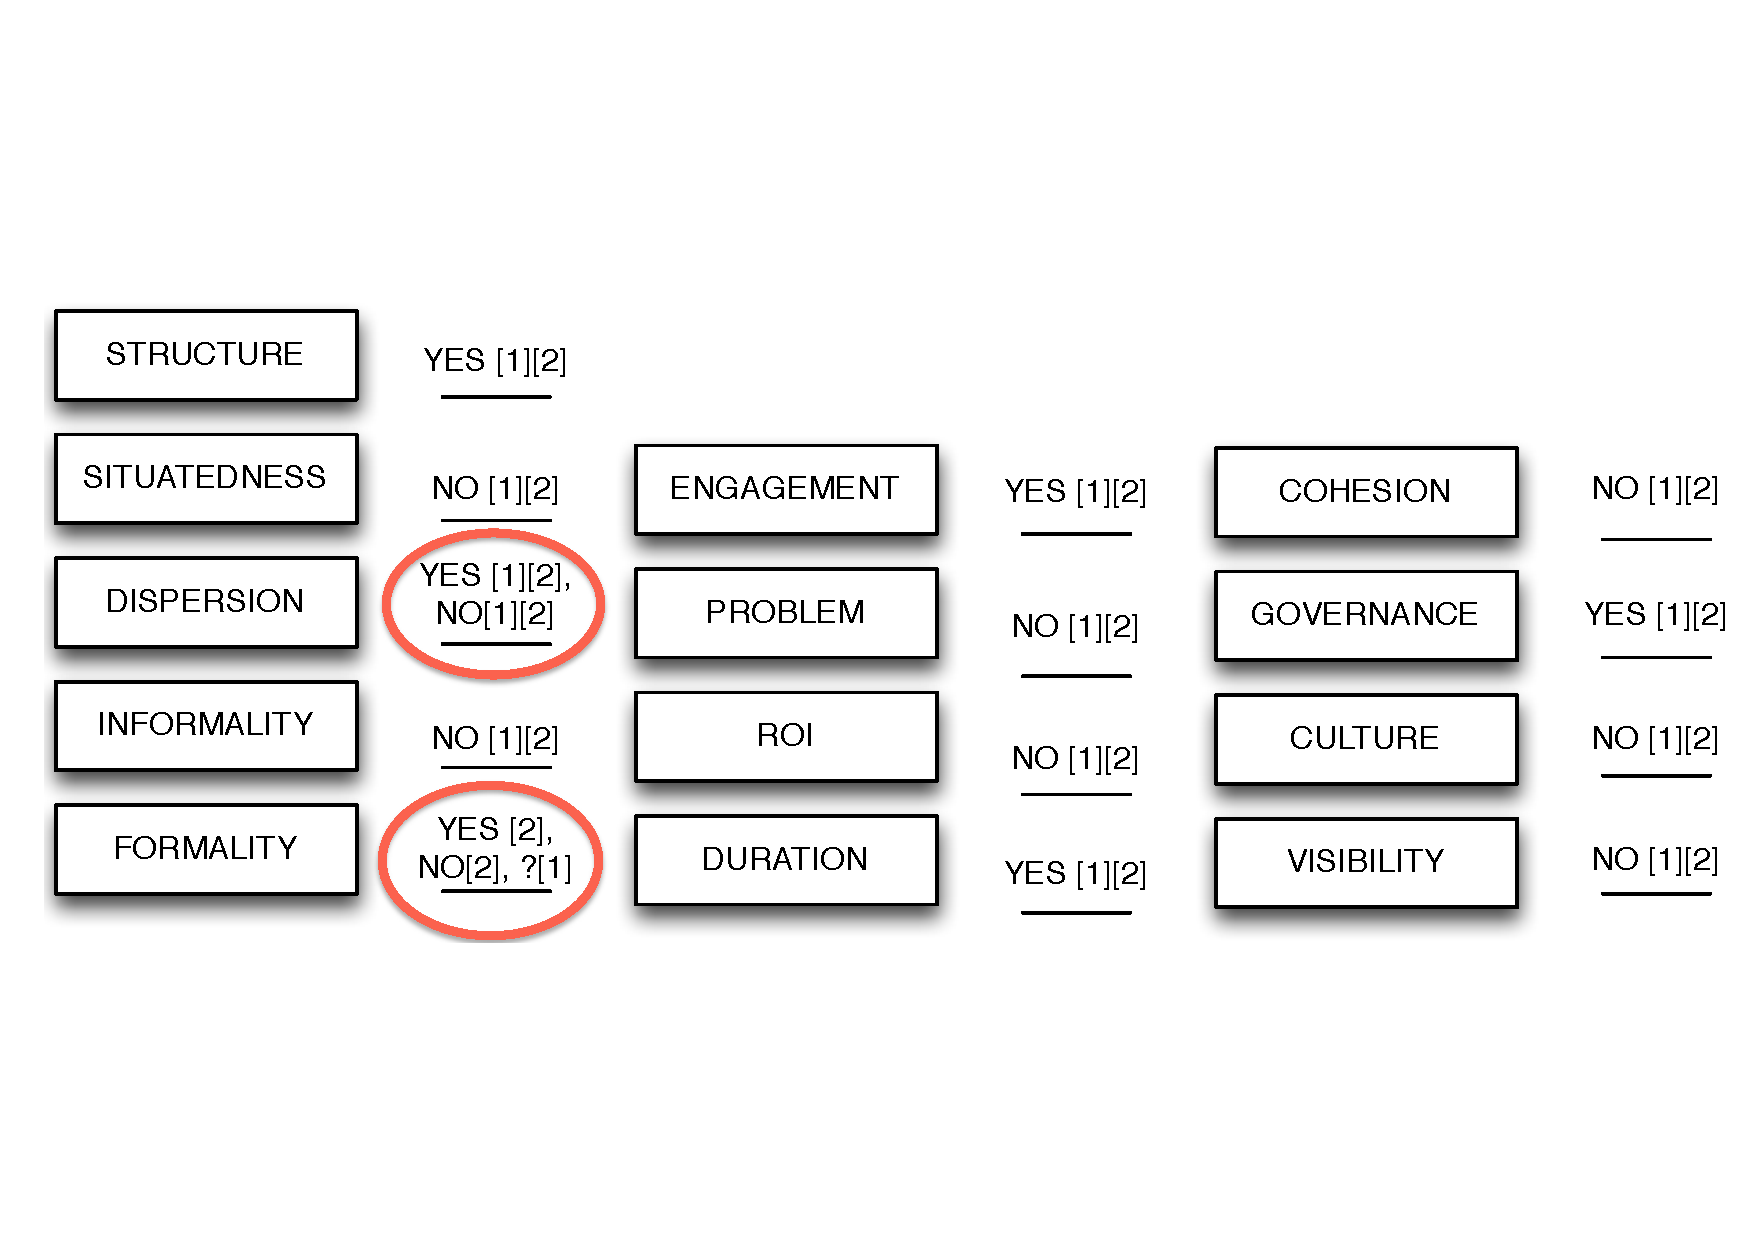
\includegraphics[width=5.4in]{checklistcase}    %
%  \end{center}
%\vspace{-.3cm}
\caption{\footnotesize SEEDS case-study: checklist.}\label{list}
%\end{wrapfigure}
\end{figure}

A deeper analysis of the checklist in Fig.~\ref{list} comparing with data from Table \ref{questionnaire} reveals two \emph{pivots} for Company X. Pivots reside, namely, in the DISPERSION and FORMALITY nodes. 
Digging deeper in the data, we found that the first \emph{pivot} DISPERSION identifies a sub-community while the second pivot identifies an inconsistency.

The first pivot, DISPERSION, is caused by the presence of two different sets of data to answer. The first set refers to Company X as a whole, describing the overall structure and operations. The second set refers to specific sites within Company X, describing their own operations, and their collaboration with open-source communities. Consequently, the specific sites work in a way different than Company X as a whole.

The second pivot, FORMALITY, is caused by an inconsistency within the observed community. While the industrial partner gave a straight YES answer to the FORMALITY question, parts of the data at our disposal led us to find that Company X did not adopt formal evaluation of members. Other parts led us to find that Company X did infact use formal procedures and background checks to enrol members in teams or other project development units. When presented with the snapshot, the industrial partner acknowledged the inconsistency. The inconsistency was due to the collaboration between open- and closed-source developers. While people directly appointed by Company X were formally evaluated, people from open-source never went through any background or experience checks.

\subsection{Applying the SEEDS Decision-tree}

Using data from the checklist (see Fig. \ref{list}) we were able to colour the SEEDS decision-tree to find emerging community types. Figure \emph{result} shows the colouring. The colouring evidences the two pivot points, namely DISPERSION and FORMALITY as well as three social communities, namely, a plain Social Network (SN), Formal Networks (FNs) and Informal Communities (ICs). Pivot points are shown in ovals, while identified social community types are shown in circles.
%(WGs - part A of Fig.~\ref{result})

According to our data, Company X is organised as a globally dispersed (i.e.~separated by distance in time and space) set of sites. No joint work sessions are planned or supported in any one site. Rather, work stays dispersed and relies on dedicated digital means for sharing and synchronisation. Overall, Company X looks like a SN, self-organising and open to collaboration with other communities. In our case, for example, some (parts of) sites, were explicitly collaborating with (and connected to) open-source communities.

The first pivot point in the DISPERSION node identifies a sub-community. The colouring reveals the sub-community to be Informal Communities (ICs), emerging in single sites. Enthusiastic engagement and collaboration both from open- and closed-source contributors are key characteristics. Frequent and formal collocated meetings are used to verify productivity. 

The second pivot point in the FORMALITY node identifies an inconsistency. Some sites work as FNs if they have no collaboration with open-source.

Our data also suggests the presence of additional ``enriching'' attributes for Company X, namely GOVERNANCE practices and DURATION.

\begin{figure}
\hspace{-.2cm}
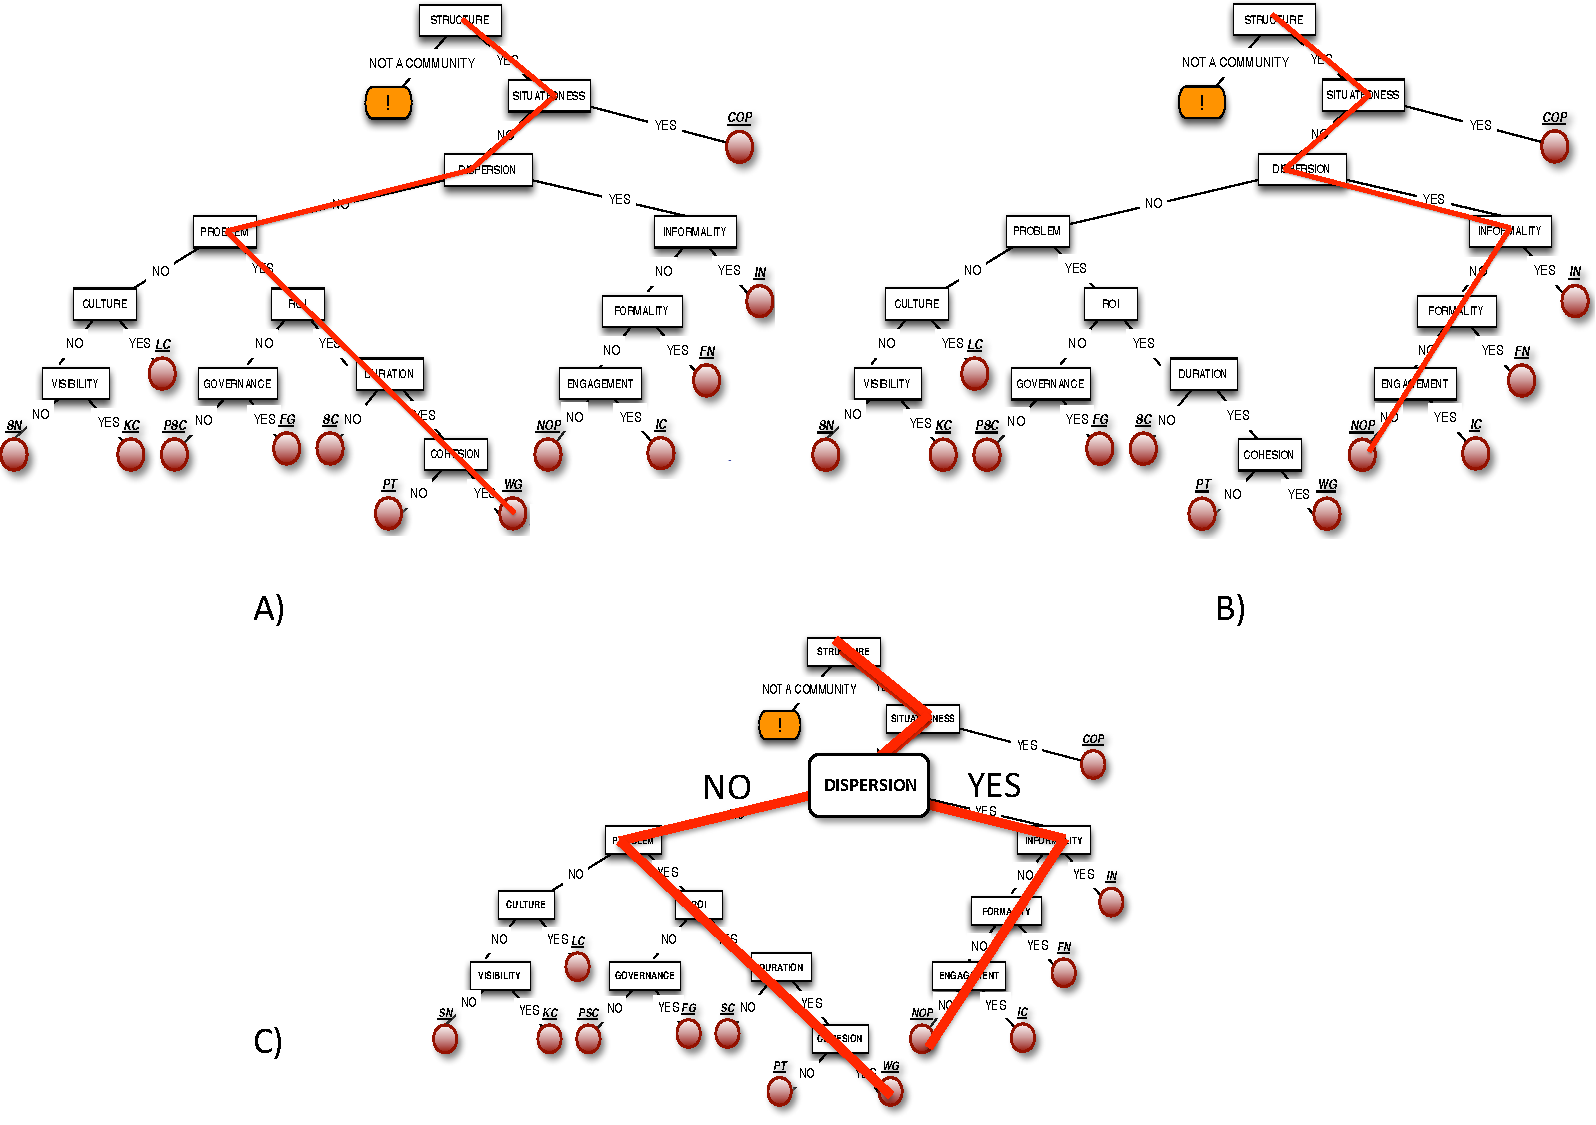
\includegraphics[width=13.4cm]{results}%
%\begin{sideways}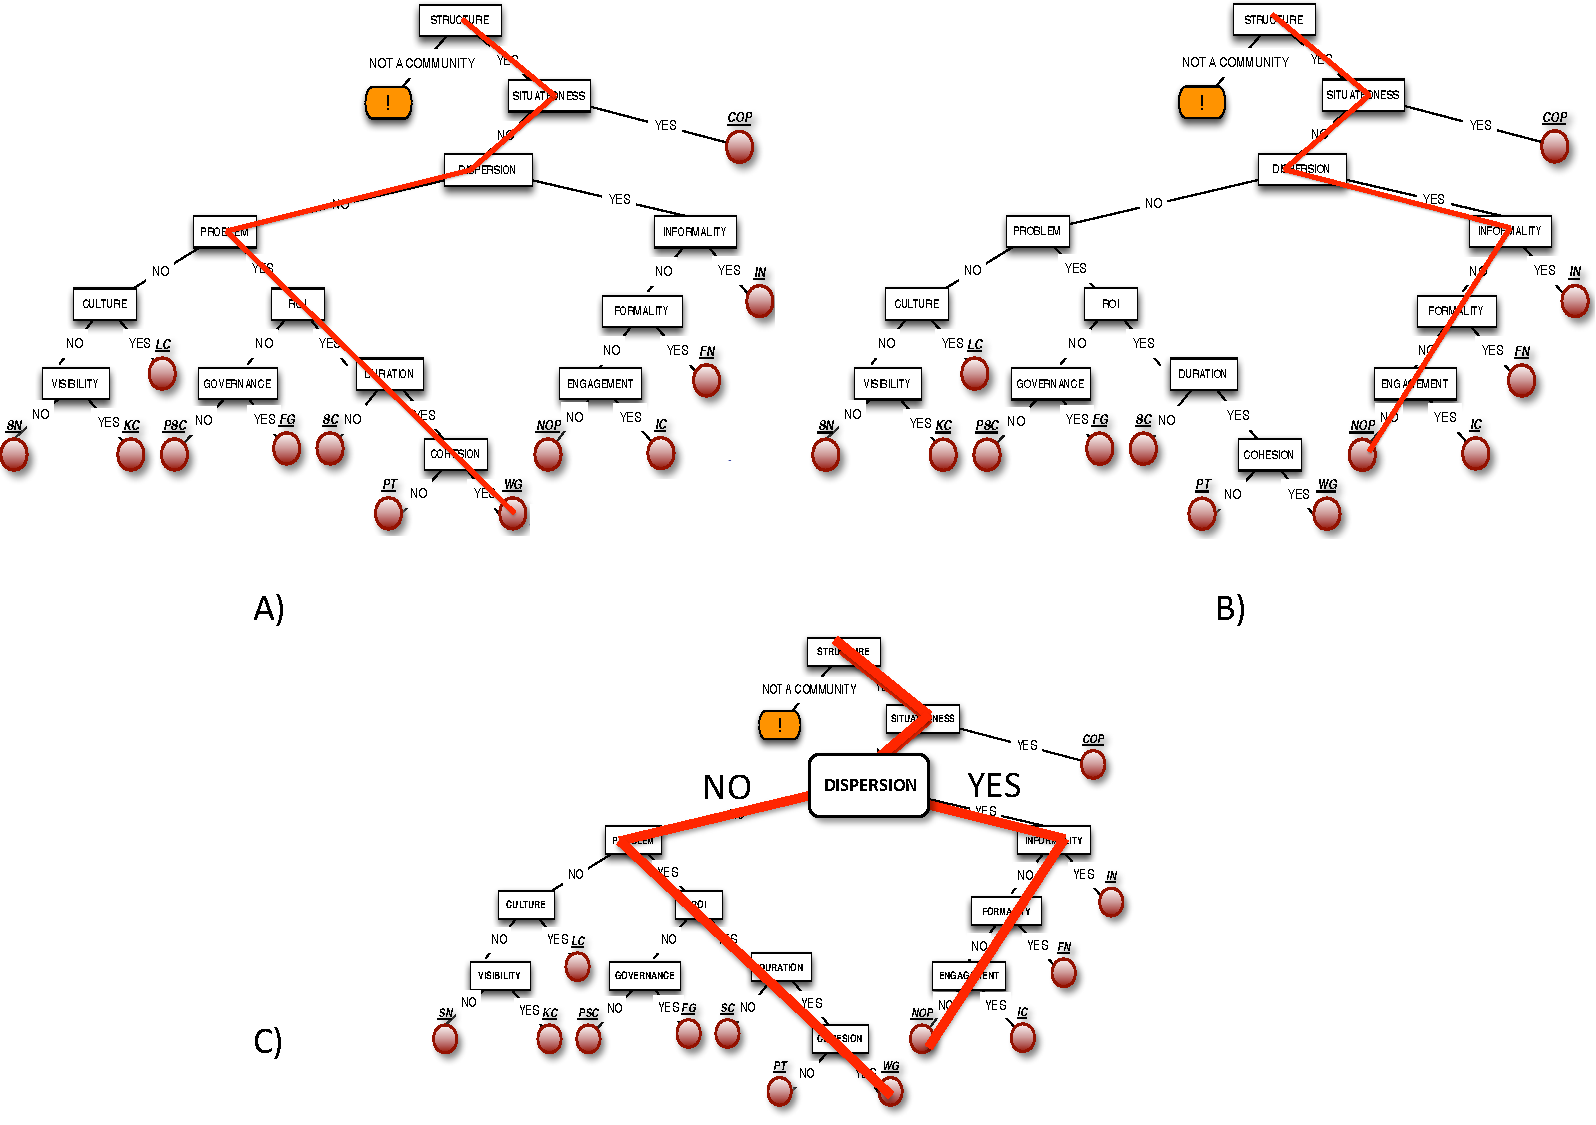
\includegraphics[width=7in]{results}\end{sideways}
\caption{SEEDS Snapshot for Company X, ovals are pivots while circles are communities found.}\label{result}
\end{figure}

\subsection{Applying the SEEDS Evaluation Framework to Diagnose Company X}

To evaluate the \emph{snapshot} we applied the SEEDS evaluation framework introduced in Section \ref{fw}. We found that Company X's \emph{snapshot} has a \emph{complex} form. The \emph{complex} form allows to identify (or confirm the identification of) the IC sub-community, involving sites that collaborate with open-source. ENGAGEMENT is the key-defining attribute of ICs. Management can explicitly support ENGAGEMENT in sites where ICs were identified.

In addition, thanks to our analysis framework we found a desirable property. The \emph{snapshot} evidences the VISIBILITY attribute set to NO. Conversely, empirical evidence from \textbf{Reference 1} and \textbf{2} indicates that members of Company X, from multiple sites, identified the need for increased VISIBILITY of practices, results, artefacts and people.

Finally, the \emph{snapshot} evidences attributes in all higher-order areas of the SEEDS decision-tree. The community at Company X does not seem to require additional steering to include missing foci.

In summary, the \emph{snapshot} allows associating Company X with the following ``diagnosis'':

\begin{enumerate}
\item \emph{\bf Three social community types are present: SNs, ICs and FNs}. While Company X looks like a SN as a whole, some sites (specifically, sites working jointly with open-source people) work as ICs. Compared to IC sites, other sites work as FNs, this can  cause inconsistencies or lack of communication/collaboration.
\item \emph{\bf Empirical evidence points to VISIBILITY as a desirable property}. Management can foster VISIBILITY as a desirable property and ENGAGEMENT as a key-defining attribute of ICs, in sites where open-source collaboration is employed.
\end{enumerate}

Using the above ``diagnosis'' and the connected \emph{snapshot}, management at Company X can have a more in-depth understanding of its social community characteristics, e.g. strengths and weaknesses.

%Based on our data, the first \emph{pivot} identifies a sub-community.
%%%% SONO ARRIVATO QUI

%%%%%%%DESIRABLE PROPERTIES:\\ USE AS EVIDENCE FOR THE LAST STEP
%%%%%%%In our case, many interviews suggested performance was hindered by an organisational barrier \cite{Correia2010}, ``lack of visibility of the whole'', meaning lack of visibility into organizational microstructures, artefacts, processes, etc. We found the \emph{snapshot} of Company X was in \emph{complex} form but the ``VISIBILITY'' attribute was set to NO. In these circumstances the creation of a Knowledge Community within Company X is beneficial to increase visibility. 

%%%%%% Martin!!! please revise/integrate!!! :)
%
%%All available evidence pointed to the identification of two community types to describe Company X, a NoP (globally) and various WGs (in Company X's sites).
%%
%%We were able to answer most questions except questions 3 and 11.
%%
%%For question 3 ``do all community members exhibit a different location?'', we found organisational information leading to both a ``YES'' or a ``NO''. Moreover, we noticed that organisational information leading to ``YES'' was related to Company X as a whole. Conversely, organisational information leading to ``NO'' was referring to only a few sites within Company X. We found that the point of indecision, i.e.~the DISPERSION node (part C of Fig.~\ref{result}) acts as a \emph{pivot} between the two community types. Attributes for the identification of a NoP were referred to global details of Company X (for these, DISPERSION was set to YES). Conversely, attributes leading to the identification of a WG were referred to localised divisions within Company X (for these, there was NO DISPERSION). 
%%
%%For question 11 ``do community members require formal status evaluation?'', it was impossible for us to answer, given the lack of available information.

%TODO: put figure of the answered questionnaire. on the figure, the pivot answers need to be with interrogation marks\\
%TODO: explain the answers\\
%%\begin{table}
%%\vspace{-4cm}
%%\hspace{-3.5cm}
%%%\begin{sideways}
%%%%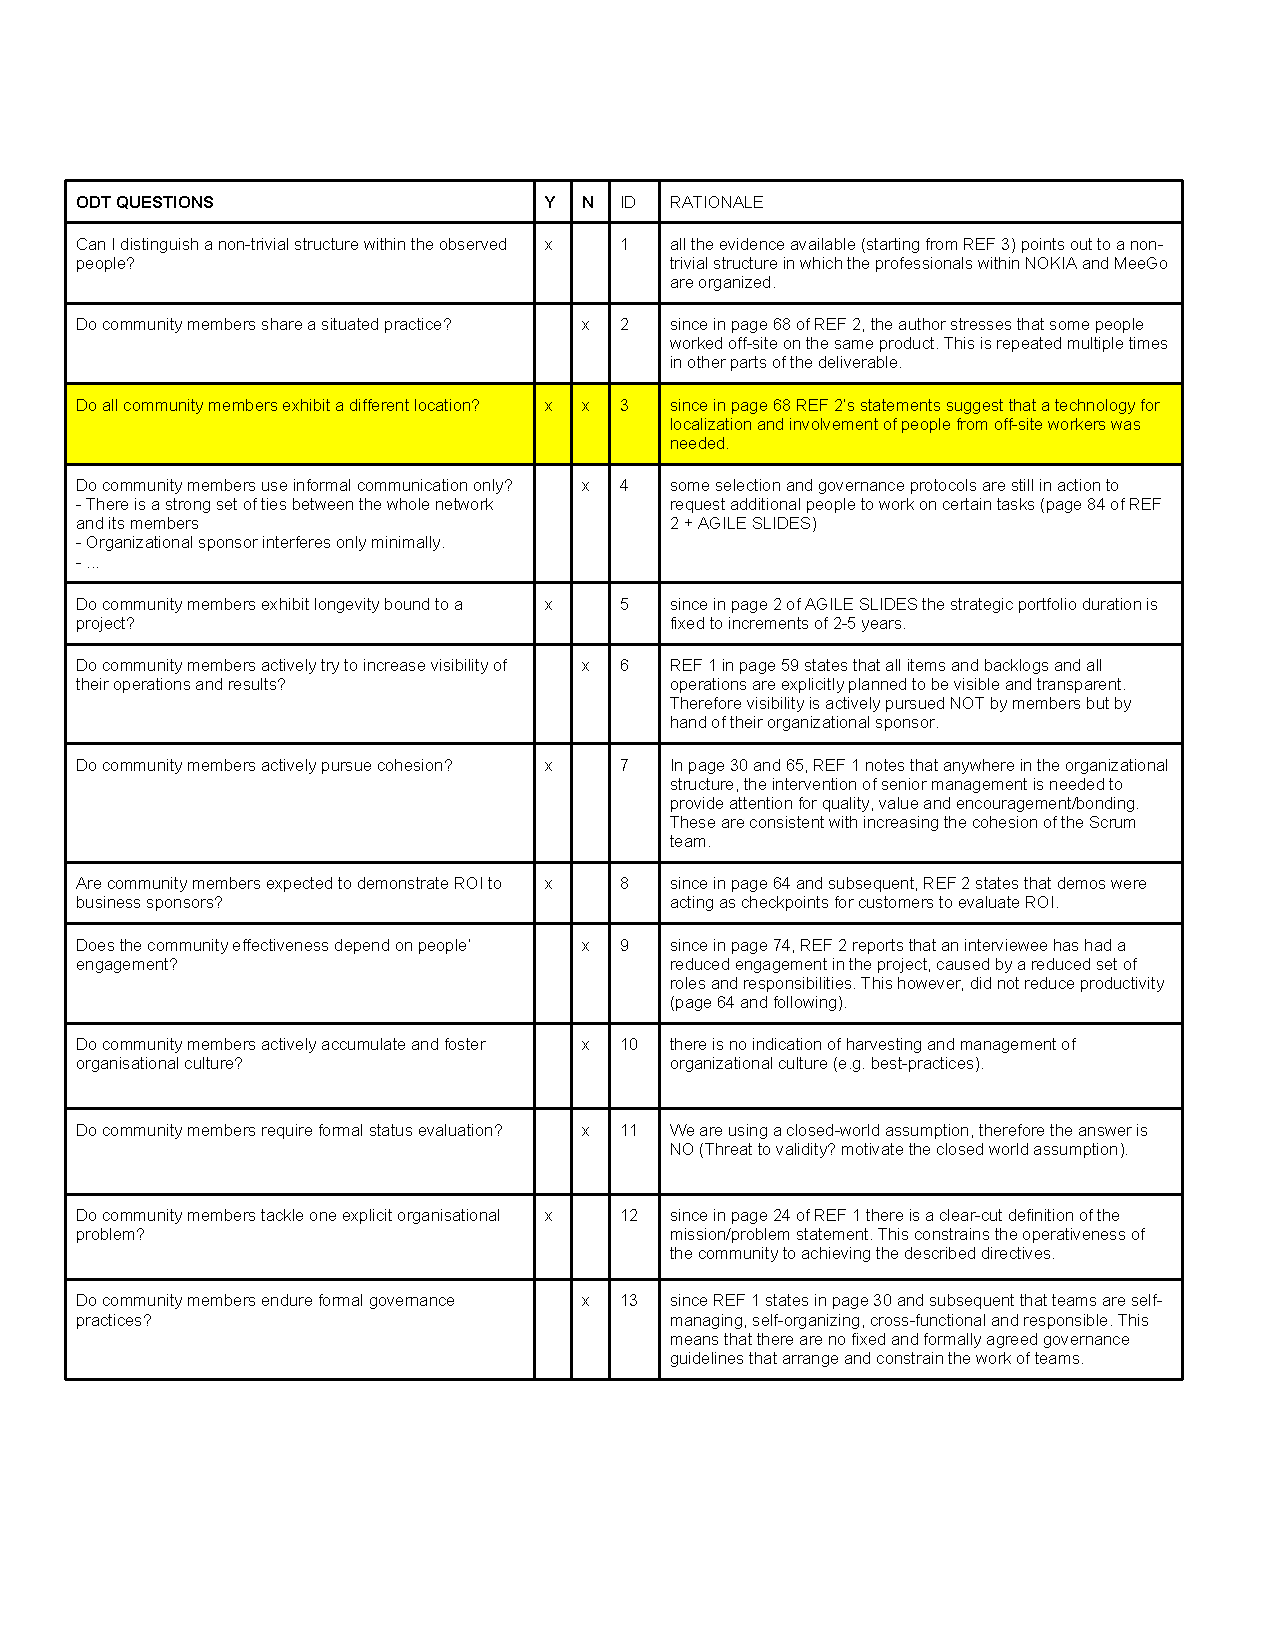
\includegraphics[width=7.5in]{answers_new}%
%%%\end{sideways}
%%\begin{tabular}{|>{\raggedright}p{4cm}|c|c|c|>{\raggedright}p{13cm}|}
%%\hline 
%%\textbf{QUESTION} & \textbf{Y} & \textbf{N} & \textbf{ID} & \textbf{RATIONALE}\tabularnewline
%%\hline 
%%Can I distinguish a non-trivial structure within the observed people? & x &  & 1 & REF 2 and3 point out to a non-trivial structure in which the professionals
%%within Company X are organized. There are divisions, products, innovation
%%areas, etc.\tabularnewline
%%\hline 
%%Do community members share a situated practice? &  & x & 2 & Page 68 of REF 2, authors stressed that some people worked off-site
%%on the same product. This is repeated multiple times in other parts
%%of the research report.\tabularnewline
%%\hline 
%%Do all community members exhibit a different location? & \multicolumn{1}{c}{} & ? & 3 & in page 68 REF 2 suggested that a technology for localization and
%%involvement of people from off-site workers was needed but not explicitly
%%present in a technological form. It follows that some components of
%%the organisational structure were indeed decentralized. However, other
%%both REF 2 and 3 speak about a collocated development process.\tabularnewline
%%\hline 
%%Do community members use informal communication only? &  & x & 4 & Rigid selection and governance protocols are in action to request
%%additional people to work on certain tasks (page 84 of REF 2 + AGILE
%%SLIDES).\tabularnewline
%%\hline 
%%Do community members exhibit longevity bound to a project? & x &  & 5 & Page 2 of AGILE SLIDES showed the strategic portfolio duration. This
%%is fixed to increments of 2-5 years.\tabularnewline
%%\hline 
%%Do community members actively try to increase visibility of their
%%operations and results?  &  & x & 6 & REF 1, page 59 stated that all production items and Scrum backlogs
%%as well as all operations are explicitly planned to be visible and
%%transparent to all working to a product. Therefore visibility is actively
%%pursued NOT by members but by hand of their organizational sponsor.\tabularnewline
%%\hline 
%%Do community members actively pursue cohesion?  & x &  & 7 & In page 30 and 65, REF 1 noted that anywhere in the organizational
%%structure, the intervention of senior management was needed and present
%%to oversee end-product quality, contract value and people encouragement/bonding.
%%This is consistent with increasing the cohesion of Scrum teams.\tabularnewline
%%\hline 
%%Are community members expected to demonstrate ROI to business sponsors?  & x &  & 8 & In page 64 and subsequent, REF 2 stated that demos phases were acting
%%as checkpoints for customers to evaluate ROI.\tabularnewline
%%\hline 
%%Does the community effectiveness depend on people\textquoteright{}
%%engagement?  &  & x & 9 & In page 74, REF 2 reported that an interviewee had a reduced engagement
%%in the project, caused by a reduced set of roles and responsibilities.
%%This however, did not reduce productivity and consequently did not
%%lower community effectiveness (page 64 and following).\tabularnewline
%%\hline 
%%Do community members actively accumulate and foster organisational
%%culture?  &  & x & 10 & there was no indication that business units or organisation were actively
%%collecting and managing organizational culture (e.g.~best-practices,
%%usage scenarios, wicked problems etc.).\tabularnewline
%%\hline 
%%Do community members require formal status evaluation? & \multicolumn{1}{c}{} & {*} & 11 & Not enough information.\tabularnewline
%%\hline 
%%Do community members tackle one explicit organisational problem?  & x &  & 12 & In page 24 of REF 1 authors stress that there is a clear-cut definition
%%of the mission/problem statement both of the organisation and its
%%business units. This constrains the operativeness of the community
%%to achieving the prescribed directives.\tabularnewline
%%\hline 
%%Do community members endure formal governance practices?  &  & x & 13 & REF 1 stated in page 30 and subsequent that teams are self-managing,
%%self-organizing, cross-functional and responsible. This means that
%%there are no fixed and formally agreed governance guidelines that
%%arrange and constrain the work of teams.\tabularnewline
%%\hline 
%%\end{tabular}
%%\caption{Company X, questionnaire with answers.}\label{answers}
%%\end{table}
%To evaluate results we mapped the answers in Figure \ref{answers} with the decision-tree from \cite{specissue}. The result of the mapping to the decision-tree is shown in Figure \ref{result}. 
%We noticed that, when mapped to the decision-tree, the point of indecision marks the start of another path on the tree, i.e.~another community. 
%The point of indecision is a \emph{pivot} decision-tree visits.
%TODO: then proceed with showing the tree visit.\\

%%Finally, we concluded the case-study by applying the decision-tree from previous work \cite{specissue}. 

%\subsection{Replication}

%\begin{figure}
%\hspace{-.2cm}
%%\begin{sideways}
%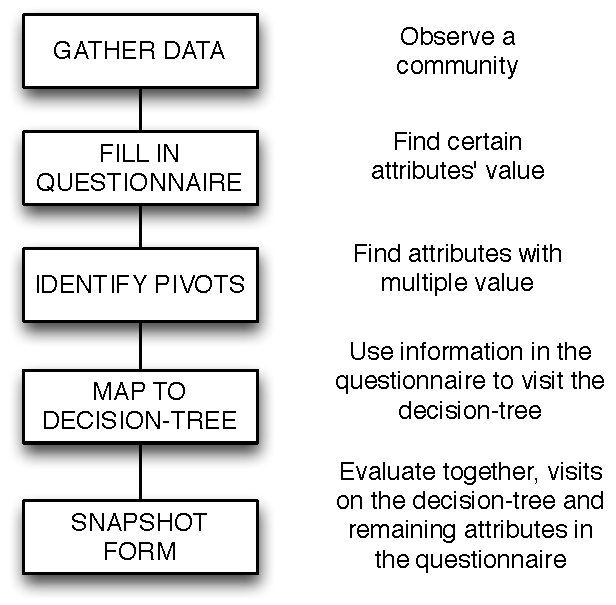
\includegraphics[width=3.5in]{method}%
%%\end{sideways}
%\caption{The SEEDS method: an overview.}\label{method}
%\end{figure}
%At this point, considerations on the \emph{snapshot} can be associated with quantitative metrics or numbers concerning the company's current organisational performance. This can be useful in both academia and industry. For academic research, it could be useful to find patterns and causal relations between metrics for organisational performance and community \emph{snapshots}, e.g.~to establish the feasibility of certain community layouts for certain organisational goals. For practitioners, this can be useful to reflect on ways in which the current organisational layout could be steered or extended to improve its performance. A process overview of the SEEDS method is shown in Fig.~\ref{method}.

%\begin{itemize}
%\item explain how the case-study was conducted
%\item explain what the evidence used to give an answer to the questionnaire
%\item show the questionnaire and the visits
%\item explain types found in the case
%\item explain the design of the case-study: (a) through a questionnaire\footnote{link to URL of SEEDSTemplate.gdoc}; (b) the decision-tree described in \cite{specissue});
%\item explain the way we had to proceed in separate cases and weekly meet to share ideas and discussion of approach only limited to clarification of tasks
%\item overseeing of two senior researchers
%\end{itemize}

% An example of a floating figure using the graphicx package.
% Note that \label must occur AFTER (or within) \caption.
% For figures, \caption should occur after the \includegraphics.
% Note that IEEEtran v1.7 and later has special internal code that
% is designed to preserve the operation of \label within \caption
% even when the captionsoff option is in effect. However, because
% of issues like this, it may be the safest practice to put all your
% \label just after \caption rather than within \caption{}.
%
% Reminder: the "draftcls" or "draftclsnofoot", not "draft", class
% option should be used if it is desired that the figures are to be
% displayed while in draft mode.
%
%\begin{figure}[!t]
%\centering
%\includegraphics[width=2.5in]{myfigure}
% where an .eps filename suffix will be assumed under latex, 
% and a .pdf suffix will be assumed for pdflatex; or what has been declared
% via \DeclareGraphicsExtensions.
%\caption{Simulation Results}
%\label{fig_sim}
%\end{figure}

% Note that IEEE typically puts floats only at the top, even when this
% results in a large percentage of a column being occupied by floats.

\section{Analysis of Results and Lessons Learned}\label{disc}
%TODO:\\
%REVISE\\
%EXTEND\\
%MARTIN WILL ADD FINDING ABOUT COMPARISON WITH THE CYNEFIN MODEL\\
%ADD FINDING ABOUT BARRIER\\
%ADD FINDING ABOUT DIFFERENT PIVOT POINT FROM TWO DISTINCT OBSERVERS\\

We analysed our results and made five key observations. The following text states the observation and provides an interpretation in \emph{italic}.

%First, the method used during the case-study can be generalised. Second, we found that the questionnaire has many uses other than gathering the needed organisational information. Second, we found that \emph{pivot} points can have multiple answers for the same community, this detail makes them worthy of particular attention. Third, we found that data in the questionnaire can assume five possible forms, each with some interesting properties. Fourth, organisational barriers can either be useful to shape an organisation or harmful to its operations. The text below explains all findings in more detail. In \emph{italic} we provide a discussion of the finding.

%\subsection{SEEDS: a method for Outlining Development Social Structures to Analyse}
%
%diversi usi della tabella:
%1. social communities multiple
%2. incompletezza? fungi da checklist
%3. ingegnerizzate una community per sw dev in forward
% inoltre, storia dei pivot e cosa significano
% inoltre, possibili forme e cosa significano

%\subsection{Findings and Observations}

%{\bf First, we found that observable organisational information misleads the detection of communities.}
%%
%\emph{This suggests that observable organisational information is overloaded with data. A questionnaire is an essential piece to organise and contain only the necessary and sufficient information to uncover a community type. In addition, this finding also suggests that some organisational information might be missing or incomplete. The questionnaire can also be used as a checklist to make sure all needed information is actually available. Finally, this finding implies that our method for community detection cannot be fully automated.}
%TODO: make examples of each of the above statements.\\


%A community \emph{snapshot} can be obtained by combining two key informations: (a) answers to the questionnaire in Fig.~\ref{quest}; (b) visits to the decision-tree from \cite{specissue}. 
%
%{\bf First, the questionnaire part of the SEEDS method� }
%TODO: finish explaining\\
%TODO: add example\\
%TODO: explain how the finding was extracted from our case study and how and why it can be generalized\\

First, Pivots can be used as drivers for the analysis of the community complexity. For example, in our case study we found evidence that led to discovering two pivot points. However, only one of them was ``by design'', i.e. was a consequence of explicit choices within the organisational structure at Company X.
%More in particular you need to visit the tree once per every possible combination of all \emph{pivots}.
\emph{This circumstance differs than finding pivots caused by explicit decisions. The more pivots are connected to implicit causes the more the community is complex and can become unmanageable, since its ``health'' is connected to circumstances and decisions that cannot be controlled or acted upon. This leads that identified pivots deserve more in-depth study by observers.}

Second, the attributes' value in the decision-tree can be determined through quantitative metrics rather than qualitative data. More complex social-network analysis (SNA) and social sensing techniques can be employed to determine more reliably or further confirm the value of attributes as needed. \emph{Snapshots are valuable tools to determine which attributes might be worthy of additional investment, e.g. through SNA. Management can delineate and ``diagnose'' their community status and use snapshots to determine which attributes should be focused-on with additional studies.}

Third, the SEEDS framework allows to uncover (un-)desirable properties and higher-order needs of a community. We found that organisational and social-networks literature defines these properties and needs as ``organisational barriers''. Barriers are mechanisms or circumstances that filter activity within a community, rephrasing Correia et al. \cite{Correia2010}. In a previous systematic literature study \cite{ossslr} we have found evidence of many ``organisational barriers''. Further research is needed to formalise barriers to allow their detection and mitigation. \emph{The work presented in this paper can be used as a lens to analyse and formalise barriers. To this purpose, for example, the SEEDS analysis framework can be improved with snapshot patterns (e.g. multiple pivots in particular points, or mismatching combinations of communities) associated to barriers.}

%%%%%%%%%%%%%%%%REVISE%%%%%%%%%%%%%%%%%%%%
% Far capire nei findings dell'articolo che cosa significano
%Che gliene frega ai practitioners? Come li aiuta? Cosa indicano? Inoltre come visualizzo uno \emph{snapshot}? Come lo contengo? Fare anche una figura del processo e mapparla sulla descrizione
%The following information couldn�t be added to Exchange:
%alert:Display message on 11/24/12 5:16 PM
%%%%%%%%%%%%%%%%%%%%%%%%%%%%%%%%%%%%%%%%%%%%%
%For example, suppose your organisational information suggests the presence of both a Formal Network (FN) and a Network-of-Practice (NoP). The pivot-point in this case is ``formality''. It follows that the community you are observing behaves formally at one level (for example on a global scale, or between sites) and informally at another level (for example between divisions or business units). It's at least something you might want to think about, if the community you are observing exhibits communication problems. Moreover, suppose you are investigating communities that should all behave in the same way. The pivot-points suggest who is diverging. You might want to consider if and why the divergence is a good thing.}
%TODO: use example of pivot from case-study\\
%
%Second, mention proof of concept since the industrial partner and our case the two sub cases revealed consistent findings and the information was correctly harvested and used, leading to the same result.

%
%\emph{These five forms can be used as a means to measure and analyse community complexity. If the community matches a single path then it's more controllable, since it refers to a single type known to literature. Steering and management complexity increases the more the observed community diverges from a simple form.}
%TODO: REVISE!!! finish explaining the fifth status and elaborate on the others; make sure that they are all\\
%TODO: add example\\
%
%Finally, organisational literature defines . We found that many barriers are present in software development communities but are not necessarily a bad thing. In our case, for example, we found the limited ``visibility of the whole'' to be an organisational barrier.  This is consistent with the community we observed in Company X. We observed a strong cooperation between Company X and open-source communities. The mechanisms we provide in this paper can aid the discovery or deployment of organisational barriers, e.g.~to increase or limit communication across (sub-)communities.
%\\
%TODO: needs the reasoning about barriers Me+Hans \\
%TODO: Add example\\
%If they are, then they constrain people's communication. 
%\section{Discussion}\label{disc}

% An example of a double column floating figure using two subfigures.
% (The subfig.sty package must be loaded for this to work.)
% The subfigure \label commands are set within each subfloat command, the
% \label for the overall figure must come after \caption.
% \hfil must be used as a separator to get equal spacing.
% The subfigure.sty package works much the same way, except \subfigure is
% used instead of \subfloat.
%
%\begin{figure*}[!t]
%\centerline{\subfloat[Case I]\includegraphics[width=2.5in]{subfigcase1}%
%\label{fig_first_case}}
%\hfil
%\subfloat[Case II]{\includegraphics[width=2.5in]{subfigcase2}%
%\label{fig_second_case}}}
%\caption{Simulation results}
%\label{fig_sim}
%\end{figure*}
%
% Note that often IEEE papers with subfigures do not employ subfigure
% captions (using the optional argument to \subfloat), but instead will
% reference/describe all of them (a), (b), etc., within the main caption.


% An example of a floating table. Note that, for IEEE style tables, the 
% \caption command should come BEFORE the table. Table text will default to
% \footnotesize as IEEE normally uses this smaller font for tables.
% The \label must come after \caption as always.
%
%\begin{table}[!t]
%% increase table row spacing, adjust to taste
%\renewcommand{\arraystretch}{1.3}
% if using array.sty, it might be a good idea to tweak the value of
% \extrarowheight as needed to properly center the text within the cells
%\caption{An Example of a Table}
%\label{table_example}
%\centering
%% Some packages, such as MDW tools, offer better commands for making tables
%% than the plain LaTeX2e tabular which is used here.
%\begin{tabular}{|c||c|}
%\hline
%One & Two\\
%\hline
%Three & Four\\
%\hline
%\end{tabular}
%\end{table}


% Note that IEEE does not put floats in the very first column - or typically
% anywhere on the first page for that matter. Also, in-text middle ("here")
% positioning is not used. Most IEEE journals/conferences use top floats
% exclusively. Note that, LaTeX2e, unlike IEEE journals/conferences, places
% footnotes above bottom floats. This can be corrected via the \fnbelowfloat
% command of the stfloats package.


\subsection{Complexity}
%%% TODO move this section to the appropriate place.

The three SEEDS \emph{snapshot} forms described in Section~\ref{fw} can also be explained in terms of the Stacey matrix \cite{sta02aa}. The matrix was introduced by Ralph Stacey to help make sense of management approaches using the two axes of ``agreement'' and ``certainty'', and is depicted in Figure~\ref{fig:stacey}.
Where certainty and agreement levels are high, decisions are \emph{simple}. However if either the certainty or agreement level drops, the situation becomes \emph{complicated}. If certainty is high but agreement is not, the situation is political; if the agreement is high but certainty is not, the situation is judgemental.

\begin{figure}[h!]
%\begin{wrapfigure}{r}{0.30\textwidth}
  \begin{center}
    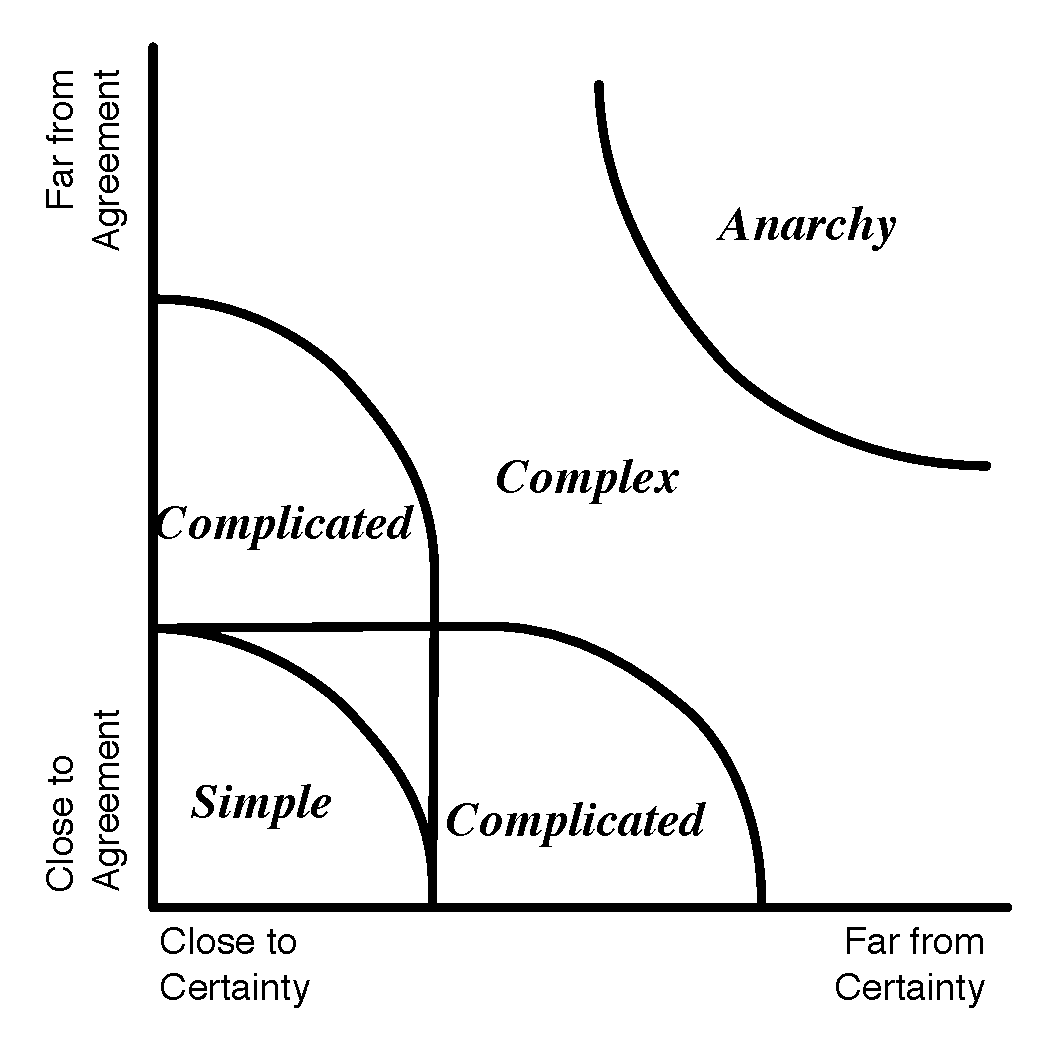
\includegraphics[width=3.4in]{Stacey.pdf}    %
  \end{center}
\vspace{-5mm}
\caption{\footnotesize The Stacey matrix (from \cite{sta02aa}.)}\label{fig:stacey}
%\end{wrapfigure}
\end{figure}

In situations where the levels of certainty and agreement are low, it may not be possible to manage and organize. This is the domain of \emph{anarchy} and chaos. Between complicated and chaos lies a large \emph{complex} area.

The three SEEDS \emph{snapshot} forms are similar, but not entirely identical, to the simple, complicated and complex domains. The SEEDS \emph{enriched-community} form represents a slight lessening of certainty and/or agreement, but does not distinguish between Stacey's two versions of complicatedness. The SEEDS \emph{complex} form implies substantially lower certainty and/or agreement.

The SEEDS model lacks an anarchic form, which is not that surprising as anarchy and chaos are antithetic to organisation.

% TODO MARTIN: expand. The 

\subsection{Method Limitations and Threats to Validity}
%%%%\begin{itemize}
%%%%\item Minna and Ossi are two different situations in two different points of Company X and different levels of abstraction. results confirmed by executing the case-study twice, contemporarily by two different researchers.
%%%%\item observations are made on only a single case-study.
%%%%\end{itemize}

While we were able to carry out a complete case-study applying SEEDS, this also taught us that the method still has many limitations. First of all, SEEDS is currently based on qualitative evidence alone. To give statistical validity to the approach, quantitative metrics should be evaluated and developed. In addition, the SEEDS analysis framework is still very preliminary and based on organisational research, rather than focused to the benefits of development communities. Testing SEEDS on working development communities gave us many insights for improvement, however much work still needs to be done. Moreover, the validation of our method through a large industrial case study, validates snapshots-based evaluation of a community, but says little or nothing about validating its evolution. Many critical research questions still remain open. For example, what is the period of time to which a snapshot should be associated? how should the SEEDS feedback loop for tuning be instrumented? Even with these limitations, our results are encouraging.

Finally, while evaluating and applying SEEDS we found some threats to validity. Based on the taxonomy in \cite{wohlin}, there are four potential validity threat areas, namely: external, construct, internal, and conclusion validity. 

\emph{``External Validity''} concerns the applicability of the results in a more general context. The validity of our conclusions could be limited to the investigated organisation. To make sure our results were generalizable we carried out a confirmatory study, focused on confirming our observations with people from Company X. The confirmatory study was also focused on assessing the (re-)applicability of our results in different contexts, based on the experience of the interviewees. The parallel confirmatory study successfully confirmed results.

\emph{``Construct Validity''} and \emph{``Internal Validity''} concern the generalizability of the constructs under study, as well as the methods used to study and analyse data (e.g.~the types of bias involved). To mitigate these threats, our methods were tailored to use multiple triangulation of data sources. A representative from Company X verified our interpretations of the data and provided clarifications and corrections where necessary. Partial results and incremental analysis was conducted to gather constant independent feedback by two senior researchers, experienced in empirical methods.

\emph{``Conclusion Validity''} concerns the degree to which our conclusions are reasonable based on our data. Our conclusions were drawn by an analysis of empirical evidence using known and confirmed methods from literature such as gap and taxonomy analysis. The approach and instruments that we used to gather such evidence were presented and validated in previous work \cite{icgseoss,icsesympo,specissue}. 

\section{Conclusion and Future Work}\label{conc}

%the paper introduced a case-study conducted to apply the method from \cite{specissue} in a real-life scenario. The case-study led us to define SEEDS a method to Outline Development Social Structures to Analyze.
%
In this paper we introduced a method to ``diagnose'' software development communities by ``snapshooting'' their state using observable attributes. The method is a refinement of previous work. To validate it we applied it on a large industrial case-study. Through many iterations we refined the method into the final version of SEEDS, a method for Snapshot-based Evaluation and Evolution of Development communitieS. This paper reports the final version of the paper and the case-study we applied it on for validation.

%We answered research question 1 (``What elements of a development community should be made explicit to study its current status?''), defining a development community \emph{snapshot} by combining: (a) answers to the questionnaire in Fig.~\ref{question}; (b) visits to the decision-tree previously introduced and (partially) validated in \cite{specissue}). This was realised by understanding that our case-study was made possible only with the presence of both elements.
%We answered research question 2 (``What are the possible forms of the development community status, or \emph{snapshot}?''), by further analysing the possible combinations that the \emph{snapshot} could present. With data from our case-study we understood what these forms meant, so that practitioners can re-apply SEEDS for their own benefit.
%We answered research question 3 (``How does organisational change influence the form of a development community \emph{snapshot}''), by sensing the presence of an organisational barrier that inhibited the effectiveness of change within Company X. 

Applying SEEDS on a large industry case-study we concluded that the method elaborates information to produce an ``actionable'' state of the community, i.e. a picture of the community that eases acting upon community characteristics. Applying the method in practice, we also recognised its many limitations. In future work we plan to explore deep into the limitations of the method, in search of improvement.

First, all our results are based on qualitative research and were applied to a single case-study. The validity of all results would benefit greatly by the presence of accompanying quantitative evidence in conjunction with multiple case-studies to increase external validity. Much work is still needed to carry out these followup studies.
We plan to establish quantitative metrics that map on the organisational complexity framework introduced in this paper. These metrics could be used by practitioners to understand community performance in numbers, e.g.~to evaluate the effectiveness of their process model in combination with the resulting community.

Moreover, additional work could be invested in demonstrating the Conway effect \cite{conway}, e.g.~by studying communities of designers and their resulting design, in a vein much similar to \cite{nachiappan}. This could be helpful in the management of architectural knowledge on a global scale.

Finally, we plan to integrate quality or process-improvement metrics in software engineering (e.g.~CMMI) with metrics and approaches to improve the development community jointly with its process. These mechanisms could be beneficial to software project management.

%TODO: explain possible followup studies, connected to the notion of community \emph{snapshot}.\\
% conference papers do not normally have an appendix

% use section* for acknowledgement
\section*{Acknowledgment}

The authors would like to thank Mr. Ossi Korhonen M.Sc. and Mrs. Minna Raisanen M.Sc. for providing empirical evidence in the form of well-defined reports, for us to elaborate the results in this paper. We acknowledge the contribution of all employees in Company X that offered their time to confirm the results contained in this paper. 

%% The Appendices part is started with the command \appendix;
%% appendix sections are then done as normal sections
%% \appendix

%% \section{}
%% \label{}

%% References
%%
%% Following citation commands can be used in the body text:
%% Usage of \cite is as follows:
%%   \cite{key}         ==>>  [#]
%%   \cite[chap. 2]{key} ==>> [#, chap. 2]
%%

%% References with bibTeX database:

\bibliographystyle{elsarticle-num}
\bibliography{comm1}

%% Authors are advised to submit their bibtex database files. They are
%% requested to list a bibtex style file in the manuscript if they do
%% not want to use elsarticle-num.bst.

%% References without bibTeX database:

% \begin{thebibliography}{00}

%% \bibitem must have the following form:
%%   \bibitem{key}...
%%

% \bibitem{}

% \end{thebibliography}


\end{document}

%%
%% End of file `elsarticle-template-num.tex'.
